\documentclass[12pt]{article}

\usepackage[margin=1in]{geometry}
\usepackage{amsmath, amssymb}
\usepackage{graphicx}
\usepackage{booktabs}
\usepackage{array}
\usepackage{caption}
\usepackage{subcaption}
\usepackage{hyperref}
\usepackage{setspace}
\usepackage{float}
\usepackage[table]{xcolor}
\usepackage{microtype}
\usepackage{enumitem}
\usepackage{natbib}

\hypersetup{
    colorlinks=true,
    linkcolor=blue!60!black,
    citecolor=blue!60!black,
    urlcolor=blue!60!black
}

\onehalfspacing

% -----------------------------------------------------------------------
% TITLE PAGE
% -----------------------------------------------------------------------

\title{\textbf{Selective Prediction and the Persistence Illusion:\\
A Diagnostic Decomposition of VIX Regime Classification}}

\author{
    Akshat Gupta\textsuperscript{1} \and
    Jianguo Liu\textsuperscript{2,*}
}

\date{}

\begin{document}

\maketitle

\noindent\textsuperscript{1} Texas Academy of Mathematics and Science, University of North Texas,
Denton, TX 76203, USA; akshatguptaakshatgupta@gmail.com; ORCID: 0009-0003-7993-1640\\
\textsuperscript{2} Department of Mathematics, University of North Texas, Denton, TX 76203, USA\\
\textsuperscript{*} Correspondence: jianguo.liu@unt.edu

\vspace{1em}
\noindent\textbf{Abstract:}
This paper develops a six-component diagnostic protocol for evaluating confidence-based
selective prediction on autocorrelated financial labels, and demonstrates it on VIX regime
classification across 5,000 trading days (July 2006--May 2026). The protocol combines
coverage-matched baseline comparison, joint-coverage decomposition, regime-transition
auditing, risk--coverage analysis, feature attribution, and abstention confound testing. Applied
to Random Forest, Histogram Gradient Boosting, and XGBoost classifiers with 36 features, the
protocol indicates that headline selective accuracy of 90--94\% largely reflects label
persistence: on jointly covered days, the Random Forest and a persistence rule calibrated on
training data make identical predictions at three of five horizons (McNemar $b = c = 0$) and
disagree on at most 3 of 708 days elsewhere. All three classifiers and a
forecast-then-threshold HAR model achieve 0\% covered accuracy on calm-to-high
transitions---across 16 distinct transition episodes at the shortest horizon---and an LSTM
performs below chance on the same days. The pattern is
consistent with an informational constraint of the daily feature set rather than a model
deficiency, and it replicates on S\&P 500 trend regimes. The protocol is modular and directly
applicable to other selective prediction systems on serially correlated outcomes.

\vspace{0.5em}
\noindent\textbf{Keywords:} VIX regime classification; selective prediction; persistence illusion;
machine learning; Random Forest; volatility forecasting; autocorrelation artifact

\vspace{0.5em}
\noindent\textbf{JEL Classification:} C53; C63; G10; G17; C12

% -----------------------------------------------------------------------
\section{Introduction}
% -----------------------------------------------------------------------

Volatility is one of the most important dimensions of financial market risk. The CBOE Volatility
Index (VIX), often described as the market's ``fear gauge,'' summarizes option-implied
expectations of S\&P 500 volatility over the next 30 days and is widely used by investors, risk
managers, and policymakers to monitor uncertainty in equity markets \citep{whaley2009,
bekaert2014}. Elevated implied volatility is both a symptom and a propagation channel of
macroeconomic uncertainty: uncertainty shocks generate sharp, clustered spikes in market fear
with real-economy consequences \citep{bloom2009}. When VIX
rises above 20---a level widely adopted as a practical divide between normal and elevated-fear
environments \citep{whaley2009}---markets are generally considered to be in a high-volatility
regime characterized by elevated fear, widening credit spreads, and increased probability of large
equity drawdowns. Episodes such as the COVID-19 crash of March 2020 and the Japan carry-trade
unwind of August 2024 illustrate the costs of failing to anticipate these regime transitions.

Despite its importance, VIX regime prediction is a difficult problem. Volatility is noisy,
mean-reverting, and driven by a complex mixture of market sentiment, equity conditions, interest
rates, and sudden exogenous shocks. Classical approaches such as GARCH-family models
\citep{bollerslev1986}, realized-volatility frameworks \citep{andersen2003}, and
Markov-switching models \citep{hamilton1989} have provided important foundations, but often
assume specific parametric structures that may not hold in practice, and macroeconomic
predictors add surprisingly little to autoregressive volatility benchmarks out of sample
\citep{paye2012}. Machine learning methods offer flexibility in modeling nonlinear
interactions across large feature sets, and have shown genuine promise in related asset
pricing applications \citep{gu2020}, but introduce their own challenges: temporal leakage,
calibration, and---critically for regime classification---the difficulty of distinguishing
genuine predictive skill from the strong autocorrelation inherent in VIX.

Before proceeding, a distinction is worth drawing explicitly: forecasting volatility itself
(a continuous quantity, the object of the GARCH and HAR literatures) and forecasting binary
volatility \emph{regimes} (whether VIX will be above a threshold at a future date) are related
but different problems. This paper is concerned with the latter---the classification task that
underlies regime-based risk dashboards, allocation switches, and hedging triggers---and with how
such classifiers should be evaluated.

The selective prediction literature---which studies classifiers that may abstain from uncertain
predictions \citep{chow1970, bartlett2008, geifman2017}---offers a principled approach to regime
classification: reserve predictions for high-confidence cases, trading coverage for reliability
on predicted days. On autocorrelated label sequences such as VIX regimes, however, selective
prediction can manufacture the appearance of skill by preferentially covering easy regime-stable
days. That persistence is hard to beat on autocorrelated financial series is well known; what is
missing from the literature is a systematic way to determine whether---and precisely
where---a given selective classifier adds anything beyond it.

The contribution of this paper is a six-component diagnostic protocol for making that
determination, together with a detailed demonstration on VIX regime classification. The protocol
comprises: (i) coverage-matched comparison against naive baselines calibrated on training data
only; (ii) decomposition of the jointly covered prediction set by regime-transition type;
(iii) transition-conditional accuracy auditing; (iv) threshold-free risk--coverage analysis;
(v) feature attribution to detect autocorrelation exploitation; and (vi) abstention confound
testing. Three ensemble classifiers---Random Forest (RF), Histogram Gradient Boosting (HGB),
and XGBoost---are trained on 36 features and abstain when calibrated probability is close
to 0.5.

Applied to this setting, the protocol indicates the following. First, headline selective
accuracy of 90--94\% is largely composition-driven: on jointly covered days, RF and a
training-calibrated persistence rule make identical predictions at three of five horizons
(McNemar $b = c = 0$) and disagree on at most 3 of 708 shared days elsewhere; the aggregate
accuracy gaps that do appear (significant only at $N = 10$, $+2.8$ pp, 95\% CI $[0.2, 5.3]$)
arise entirely from differences in \emph{which} days each system covers. Second, a HAR-style
logistic regression using only three features (current VIX level, 5-day VIX mean, 20-day VIX
mean) is statistically indistinguishable from the full 36-feature RF at matched coverage
(bootstrap CIs on the gap include zero), suggesting the additional 33 features contribute
little. Third, the confidence filter yields 0\% accuracy on every covered calm$\to$high
transition---across 16 distinct transition episodes at $N = 5$---for all three ensemble
classifiers and for a forecast-then-threshold HAR model, while an LSTM performs below chance
on the same days; explicit cost-weighting up to $20{\times}$ does not change this. Fourth, at $N = 25$, balanced accuracy collapses to
50\% for RF and HGB. Fifth, persistence at matched coverage dominates RF selective prediction
on cost-weighted utility whenever false negatives are more costly than false alarms
($C \geq 5$) at $N = 10$.

We state the scope of these claims carefully. The evidence presented here demonstrates the
persistence illusion for two highly persistent financial classification problems (VIX regimes
and S\&P 500 trend regimes); the broader proposition---that selective prediction on any
sufficiently autocorrelated label sequence is subject to the same artifact---is a hypothesis
for which this study provides the first two supporting cases, not a demonstrated general
property.

The remainder of the paper is organized as follows. Section~\ref{sec:related} reviews related
work. Section~\ref{sec:data} describes the data. Section~\ref{sec:methodology} presents the
methodology. Section~\ref{sec:results} reports empirical results. Section~\ref{sec:replication}
replicates the diagnostic on S\&P 500 trend regimes. Section~\ref{sec:conclusion} concludes.

% -----------------------------------------------------------------------
\section{Related Work}
\label{sec:related}
% -----------------------------------------------------------------------

\subsection{Volatility Forecasting and Regime Modeling}

The modeling of financial volatility has a long history in econometrics.
\citet{bollerslev1986} introduced the GARCH model, which captures the tendency of volatility
to cluster over time by modeling conditional variance as a function of past squared residuals.
GARCH-family models have since been extended in numerous directions and remain a standard
benchmark for volatility forecasting. \citet{hamilton1989} introduced Markov-switching models,
in which a time series is assumed to switch between discrete latent states according to a Markov
chain. This framework provides a natural model for regime transitions and has been widely applied
to financial and macroeconomic time series. \citet{guidolin2007} extended regime-switching ideas
to multivariate portfolio allocation settings, demonstrating that regime-dependent models can
outperform single-state specifications in out-of-sample asset allocation.

A complementary strand of work focuses on realized volatility constructed from high-frequency
intraday returns \citep{andersen2003}. \citet{corsi2009} proposed the Heterogeneous Autoregressive (HAR) model, which
captures the long-memory properties of realized volatility through a simple additive structure of
daily, weekly, and monthly volatility components. The HAR model has become a standard benchmark
for realized volatility forecasting, and its strong performance motivates including a HAR-style
logistic regression as a baseline in this paper.

In the VIX-specific literature, \citet{whaley2009} documented the VIX's role as a fear indicator
and its asymmetric behavior in market downturns. \citet{bekaert2014} decompose the VIX into a
conditional-variance component and a variance risk premium, showing the two carry distinct
information about risk appetite and uncertainty. \citet{fernandes2014} studied the predictability
of VIX using a variety of econometric models and found that simple autoregressive specifications
perform competitively against more complex alternatives. This paper replicates and extends that
finding: simple HAR-style models are competitive with 36-feature ensemble classifiers on the
binary regime classification task.

\subsection{Machine Learning for Financial Prediction}

Machine learning methods have increasingly been applied to financial forecasting.
\citet{gu2020} provide the benchmark demonstration for empirical asset pricing, showing that
tree ensembles and neural networks extract genuine predictive gains from large predictor sets.
Ensemble methods such as Random Forests \citep{breiman2001} and Gradient Boosting are
particularly well-suited to financial prediction because they can model nonlinear interactions
among large feature sets without requiring distributional assumptions. The present paper's
message is complementary rather than contradictory to this literature: flexible models can add
value, but on highly persistent classification targets their apparent gains require the kind
of persistence-matched auditing developed here.

A key methodological challenge in applying machine learning to financial data is avoiding data
leakage and respecting the temporal ordering of observations. This paper addresses this by using
chronological train/test splitting, \texttt{TimeSeriesSplit} cross-validation during calibration,
and walk-forward validation as a robustness check---consistent with best practices in applied
financial machine learning.

\subsection{Selective Prediction and the Reject Option}

The reject option in classification allows a model to abstain from making a prediction when its
confidence is insufficient. \citet{chow1970} first formalized the optimal reject option.
\citet{bartlett2008} studied classification with a reject option using hinge loss and established
theoretical generalization bounds. \citet{geifman2017} demonstrated that selective prediction
can substantially improve reliability in modern deep learning settings.

A subsequent literature has developed evaluation methodology specifically for selective
classifiers. \citet{elyaniv2010} laid theoretical foundations for the risk--coverage trade-off,
characterizing the achievable frontier between abstention rate and selective error.
\citet{geifman2019} proposed the area under the risk--coverage curve (AURC) as a threshold-free
summary of selective performance, now a standard reporting convention. \citet{fisch2022}
extended calibration requirements to the selective setting, noting that confidence scores must
remain calibrated conditional on coverage. This evaluative strand is directly relevant here:
the diagnostic protocol we propose can be viewed as extending risk--coverage evaluation with
components that are specifically needed when labels are serially correlated---transition-type
decomposition, joint-coverage composition analysis, and persistence-matched baselines.

In financial applications, the reject option is particularly natural. A risk model that provides
no signal on ambiguous days is often more useful than one that forces a low-confidence prediction.
However, on autocorrelated series such as VIX regimes, abstention can manufacture accuracy without
genuine predictive skill---the central diagnostic this paper examines.

% -----------------------------------------------------------------------
\section{Data}
\label{sec:data}
% -----------------------------------------------------------------------

\subsection{Market Data}

Daily price data are obtained from Yahoo Finance for eight market series: the CBOE Volatility
Index (VIX), the 3-month VIX term structure index (VIX3M), the CBOE 9-Day Volatility Index
(VIX9D), the S\&P 500 Index, gold futures (GC=F), the 10-Year Treasury Yield (TNX), the U.S.\
Dollar Index (DXY), and the CBOE SKEW Index. VIX9D is downloaded to keep the raw data complete
but is not used as a model feature. Although raw VIX data is available from January 1990, VIX3M
data begins in July 2006; because VIX3M anchors the term spread feature, the effective sample
starts on July 17, 2006.

\subsection{Macroeconomic Data}

Two macroeconomic variables are obtained from the Federal Reserve Economic Data (FRED) API: the
Federal Funds Rate and the 10-Year minus 2-Year Treasury yield curve spread (T10Y2Y). The Federal
Funds Rate target is forward-filled to daily frequency by holding the prevailing rate constant
between FOMC meeting dates.

\subsection{Label Construction}

The prediction task is binary regime classification. For a prediction horizon $N$, the label is:
\begin{equation}
    \text{LABEL}_{N,t} = \begin{cases} 1 & \text{if } \text{VIX}_{t+N} \geq 20 \\ 0 & \text{if } \text{VIX}_{t+N} < 20 \end{cases}
    \label{eq:label}
\end{equation}

The label is forward-shifted $N$ days to ensure that all features are observed at time $t$ and
the outcome is measured at time $t + N$, eliminating lookahead bias. Horizons
$N \in \{5, 10, 15, 20, 25\}$ trading days are evaluated.

The threshold of 20 follows the long-standing practitioner convention documented by
\citet{whaley2009}: it sits close to the long-run VIX median, is the level most commonly used
in industry commentary and risk dashboards to separate ``normal'' from ``elevated-fear''
environments, and is embedded in numerous volatility-targeting product rules. It is
nonetheless a convention rather than a structural break point, so robustness at thresholds of
18 and 22 is reported in Appendix~\ref{app:robustness}, and we note that data-driven threshold
selection (e.g., from a fitted regime-switching model) is a reasonable alternative that would
change class prevalence but not the diagnostic design.

A \emph{sustained-high} label is also constructed:
\begin{equation}
    \text{SUSTAINED\_LABEL}_{N,t} = \begin{cases} 1 & \text{if } \text{VIX}_{t+k} \geq 20 \;\text{for all}\; k \in \{1, \ldots, N\} \\ 0 & \text{otherwise} \end{cases}
    \label{eq:sustained}
\end{equation}

\subsection{Class Distribution and Train/Test Split}

The full feature dataset covers 5,000 trading days from July 17, 2006 to May 29, 2026. Data
are split chronologically, with the first 80\% used for training (2006--2022) and the remaining
20\% for testing (2022--2026), preserving strict temporal ordering.

\begin{table}[H]
\centering
\caption{Sample sizes and class distribution (fraction of days with VIX $\geq$ 20) by
prediction horizon after label shifting. The usable sample shrinks slightly with $N$ because
the final $N$ days of the series have no observable label.}
\label{tab:class}
\begin{tabular}{ccccc}
\toprule
$N$ & Train $N$ & Test $N$ & Train VIX $\geq$ 20 & Test VIX $\geq$ 20 \\
\midrule
5  & 3,996 & 999 & 36.7\% & 30.1\% \\
10 & 3,992 & 998 & 36.7\% & 30.1\% \\
15 & 3,988 & 997 & 36.8\% & 30.0\% \\
20 & 3,984 & 996 & 36.8\% & 29.9\% \\
25 & 3,980 & 995 & 36.9\% & 29.8\% \\
\bottomrule
\end{tabular}
\end{table}

High-volatility days are substantially less common in the test period ($\approx$30\%) than in
training ($\approx$37\%), reflecting that the training window encompasses several high-volatility
crises---the 2008--09 financial collapse, the 2011 eurozone episode, and the COVID-19 crash---
whereas the test window is dominated by the post-bear-market recovery despite the elevated
volatility of the first half of 2022. The majority-class (always-calm) baseline therefore
achieves approximately 70\% accuracy on the test window before any model is fit.

% -----------------------------------------------------------------------
\section{Methodology}
\label{sec:methodology}
% -----------------------------------------------------------------------

\subsection{Feature Engineering}

The model uses 36 engineered features grouped into five categories. All features are computed
using only information available at or before the prediction date $t$.

\textbf{VIX technical indicators} (13 features): 10-day and 20-day simple moving averages
(SMA10, SMA20); 10-day and 20-day momentum; 10-day and 20-day rate of change; Bollinger Band
standard deviation, upper and lower bands, and position within the band; 14-day RSI;
moving-average cross (SMA10 $-$ SMA20); and VIX term spread (VIX3M $-$ VIX).

\textbf{SKEW features} (3 features): SKEW level, 5-day change, and 20-day change.

\textbf{S\&P 500 features} (7 features): 1-day, 5-day, and 20-day returns; 10-day and 20-day
price momentum; 20-day realized volatility; and 252-day maximum drawdown.

\textbf{Cross-asset features} (9 features): Gold 1-day, 5-day, and 20-day returns; 10-Year
Treasury Yield 1-day, 5-day, and 20-day changes; DXY 1-day, 5-day, and 20-day returns.

\textbf{Macroeconomic features} (4 features): Federal Funds Rate 1-month and 3-month changes;
yield curve spread 1-month and 3-month changes.

The complete feature list appears in Appendix~\ref{app:features}.

\subsection{Models and Training Pipeline}

Three ensemble classifiers are evaluated: Random Forest (RF) and Histogram Gradient Boosting
(HGB), both implemented via scikit-learn, and XGBoost \citep{chen2016}. All use a single fixed
specification: RF with \texttt{n\_estimators=200}, \texttt{max\_depth=10},
\texttt{min\_samples\_leaf=5}; HGB with \texttt{max\_iter=200}, \texttt{max\_depth=5},
\texttt{learning\_rate=0.1}; XGBoost with \texttt{n\_estimators=200}, \texttt{max\_depth=6},
\texttt{learning\_rate=0.1}, \texttt{subsample=0.8}, and
\texttt{colsample\_bytree=0.8}. All seeds set to \texttt{random\_state=42}. Using one specification eliminates pipeline inconsistencies
and provides a fair comparison across tables. All features are standardized using
\texttt{StandardScaler} fit on the training set and applied to the test set. XGBoost is run
through the identical pipeline (same features, split, calibration, and abstention rule) so that
its transition-level behavior is directly comparable to RF and HGB.

\subsection{Probability Calibration}

The selective prediction rule requires well-calibrated probability estimates. We apply isotonic
regression calibration using \texttt{CalibratedClassifierCV} with 5-fold
\texttt{TimeSeriesSplit} cross-validation on the full training set. The calibrated probability
at time $t$ is denoted $\hat{p}_t$, representing the estimated probability that VIX will be in a
high-volatility regime at $t + N$.

\subsection{Confidence-Based Selective Prediction}

The selective classifier makes a prediction only when $\hat{p}_t$ is sufficiently far from 0.5.
For confidence threshold $\tau \in (0, 0.5)$, the prediction rule is:
\begin{equation}
    \hat{y}_t = \begin{cases}
        1 & \text{if } \hat{p}_t > 0.5 + \tau \\
        0 & \text{if } \hat{p}_t < 0.5 - \tau \\
        \text{abstain} & \text{if } 0.5 - \tau \leq \hat{p}_t \leq 0.5 + \tau
    \end{cases}
    \label{eq:selective}
\end{equation}

Accuracy is evaluated only on days where the model makes a prediction. Coverage is defined as
the fraction of test days on which a prediction is made. The primary threshold is $\tau = 0.25$.

% -----------------------------------------------------------------------
\section{Results}
\label{sec:results}
% -----------------------------------------------------------------------

\subsection{Main Accuracy Results}
\label{sec:main}

Table~\ref{tab:main} reports baseline and selective accuracy, coverage, and balanced accuracy
on covered days at $\tau = 0.25$.

\begin{table}[H]
\centering
\caption{Baseline and selective ($\tau = 0.25$) accuracy, coverage, and balanced accuracy on
covered days. Gain = selective minus baseline in percentage points (pp).}
\label{tab:main}
\resizebox{\textwidth}{!}{%
\begin{tabular}{cccccccccc}
\toprule
$N$ & RF Base & RF Sel & RF Gain & RF Cov & RF BalAcc & HGB Sel & HGB Gain & HGB Cov & HGB BalAcc \\
\midrule
5  & 83.4\% & 91.9\% & $+$8.5 pp & 76.3\% & 88.4\% & 92.1\% & $+$8.9 pp & 71.1\% & 88.2\% \\
10 & 79.5\% & 90.0\% & $+$10.5 pp & 60.1\% & 84.8\% & 92.2\% & $+$13.6 pp & 63.1\% & 86.1\% \\
15 & 76.2\% & 90.0\% & $+$13.8 pp & 51.3\% & 83.9\% & 92.2\% & $+$21.3 pp & 36.0\% & 89.5\% \\
20 & 76.8\% & 92.7\% & $+$15.9 pp & 31.7\% & 79.1\% & 94.8\% & $+$22.2 pp & 26.8\% & 84.1\% \\
25 & 73.4\% & 90.3\% & $+$16.9 pp & 26.9\% & \textbf{50.0\%} & 92.7\% & $+$26.5 pp & 19.2\% & \textbf{50.0\%} \\
\bottomrule
\end{tabular}}
\end{table}

\begin{table}[H]
\centering
\caption{Extended metrics on covered days for Random Forest ($\tau = 0.25$). At $N = 25$,
precision and recall are both 0\% and balanced accuracy equals 50\%, confirming the model
exclusively predicts the calm class at this horizon.}
\label{tab:extended}
\begin{tabular}{cccccc}
\toprule
$N$ & Selective Acc & Precision & Recall & F1 & Balanced Acc \\
\midrule
5  & 91.9\% & 86.5\% & 81.2\% & 83.8\% & 88.4\% \\
10 & 90.0\% & 86.8\% & 73.8\% & 79.7\% & 84.8\% \\
15 & 90.0\% & 89.8\% & 70.8\% & 79.2\% & 83.9\% \\
20 & 92.7\% & 100.0\% & 58.2\% & 73.6\% & 79.1\% \\
25 & 90.3\% & 0.0\% & 0.0\% & 0.0\% & \textbf{50.0\%} \\
\bottomrule
\end{tabular}
\end{table}

\begin{figure}[H]
    \centering
    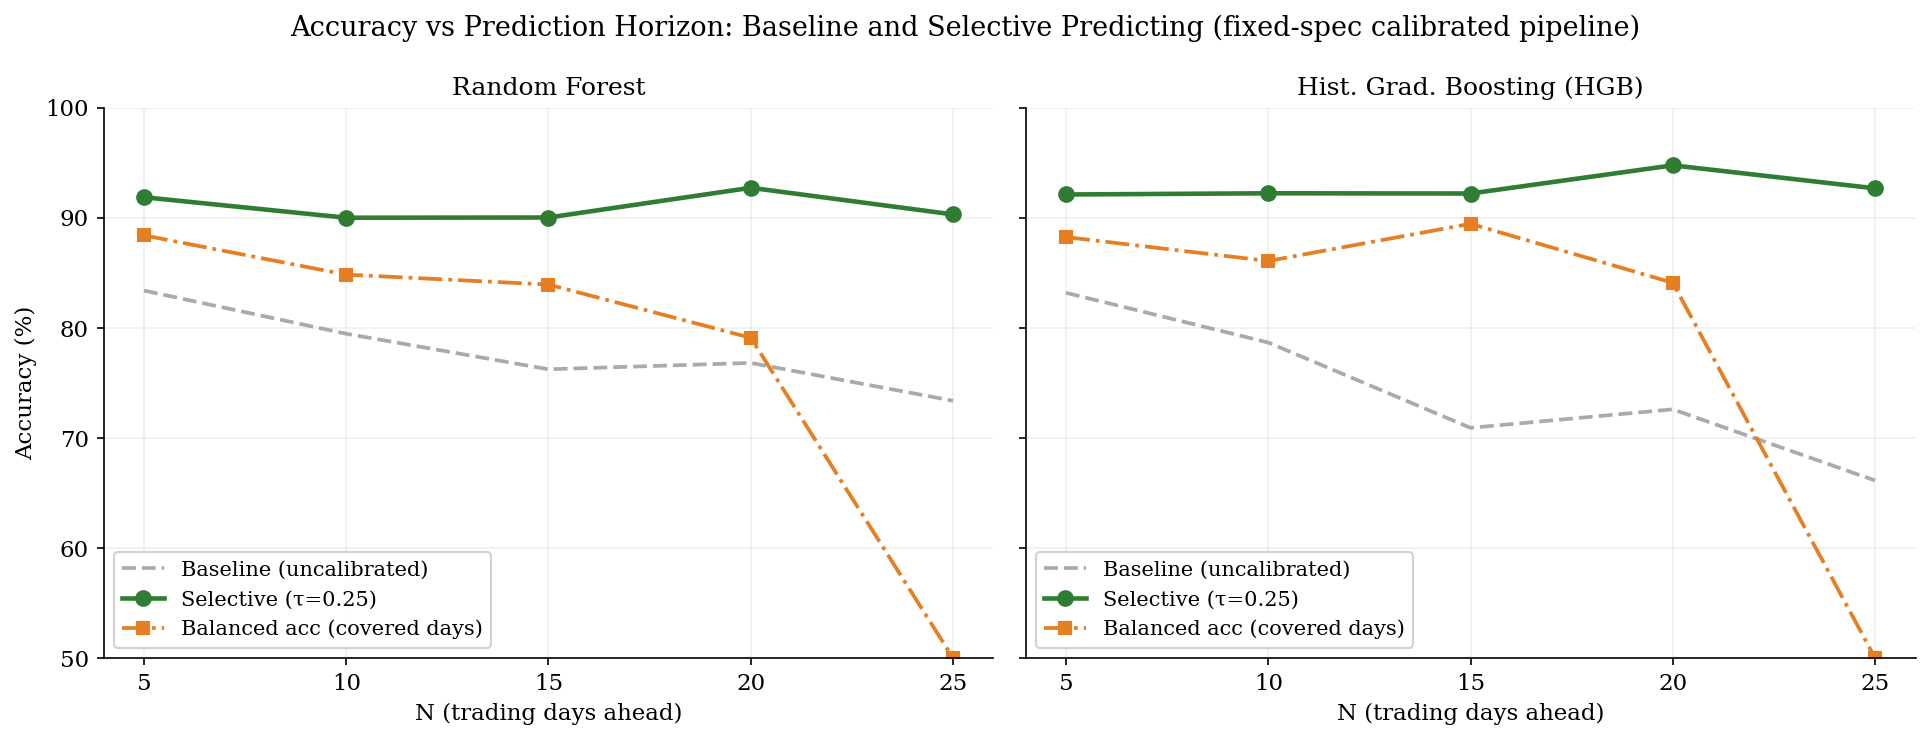
\includegraphics[width=0.85\textwidth]{tuned_model_comparison.png}
    \caption{Baseline, selective accuracy, and balanced accuracy across prediction horizons for
    Random Forest (left) and HGB (right). Baseline accuracy is computed on all test days;
    selective and balanced accuracy on covered days only. At $N = 25$, balanced accuracy equals
    50\%, indicating a coin-flip result despite 90\% selective accuracy.}
    \label{fig:main}
\end{figure}

Selective prediction improves accuracy for both models at every horizon. The balanced-accuracy
columns, however, reveal the underlying artifact: RF balanced accuracy declines monotonically
to 50.0\% at $N = 25$, indicating that the model exclusively predicts calm outcomes at the
longest horizon---the nominal 90\% selective accuracy there reflects the 70\% base rate of
calm days, not predictive skill.

\subsection{Comparison to Naive Baselines}
\label{sec:baselines}

A critical question is whether the RF selective accuracy reflects genuine multi-feature ML skill
or simply VIX autocorrelation. To answer this, we construct four coverage-matched baselines
evaluated on the same test set.

The \textbf{persistence baseline} predicts $\text{VIX}_{t+N} \geq 20$ if and only if
$\text{VIX}_t \geq 20$, and abstains when $|\text{VIX}_t - 20| < c$. The constant $c$ is
calibrated on the \emph{training window only}: we compute the RF's coverage rate on the
training set at $\tau = 0.25$ and select the smallest $c$ whose training-window coverage
matches it, then freeze $c$ and apply it unchanged to the test window. No test-set
information---neither labels nor VIX levels---enters the choice of $c$. The same protocol is
used for every coverage-matched baseline below: each baseline's abstention threshold is set as
the quantile of its own training-window confidence distribution that reproduces the RF's
training coverage rate, then frozen. Because the thresholds are frozen before the test window
is touched, realized test coverage rates differ modestly across systems (persistence covers
81.4\% vs.\ the RF's 76.3\% at $N = 5$, and 21.2\% vs.\ 26.9\% at $N = 25$); we report both
rates and address the composition of the covered sets directly in
Section~\ref{sec:joint_coverage}.

The \textbf{LR (VIX only) baseline} applies the full calibration
pipeline to a single feature (current VIX level). The \textbf{HAR-style logistic regression}
uses three features motivated by the HAR model \citep{corsi2009}: current VIX ($\text{VIX}_D$),
5-day VIX mean ($\text{VIX}_W$), and 20-day VIX mean ($\text{VIX}_M$). The
\textbf{Markov-chain baseline} estimates the 1-step transition probability matrix from training
data and raises it to the $N$th power.

\begin{table}[H]
\centering
\caption{RF selective accuracy vs.\ naive baselines ($\tau = 0.25$; all baseline abstention
thresholds calibrated on the training window and frozen). All accuracies are computed on each
system's covered test days. Cov columns report realized test coverage. Bolded values indicate
where a baseline exceeds the RF selective accuracy.}
\label{tab:baselines}
\resizebox{\textwidth}{!}{%
\begin{tabular}{ccccccccc}
\toprule
$N$ & RF Cov & Persist Cov & Persistence & LR (VIX) & HAR-LR & Markov & RF Sel & RF$-$Persist \\
\midrule
5  & 76.3\% & 81.4\% & 90.2\% & 91.8\% & 90.7\% & 83.7\% & 91.9\% & $+$1.7 pp \\
10 & 60.1\% & 71.1\% & 87.2\% & 87.6\% & 87.8\% & 78.8\% & 90.0\% & $+$2.8 pp \\
15 & 51.3\% & 64.1\% & 85.6\% & 88.4\% & 88.2\% & 70.0\% & 90.0\% & $+$4.4 pp \\
20 & 31.7\% & 45.7\% & 88.6\% & 87.9\% & 90.3\% & 84.5\% & 92.7\% & $+$4.2 pp \\
25 & 26.9\% & 21.2\% & 82.9\% & 86.8\% & \textbf{90.8\%} & 82.9\% & 90.3\% & $+$7.4 pp \\
\bottomrule
\end{tabular}}
\end{table}

\begin{figure}[H]
    \centering
    
\includegraphics[width=0.85\textwidth]{persistence_baseline.png}
    \caption{Left: RF selective vs.\ naive baseline accuracy across horizons (covered test days;
    baseline thresholds frozen from the training window). Right: RF-minus-persistence gap with
    95\% moving-block bootstrap CI; only the $N = 10$ interval excludes zero.}
    \label{fig:baselines}
\end{figure}

Three observations follow from Table~\ref{tab:baselines}. First, the HAR-style logistic
regression---using only three VIX-related features---remains within 1--4 pp of the full
36-feature RF at every horizon and exceeds it at $N = 25$. A moving-block bootstrap on the
HAR-minus-RF gap yields 95\% CIs that include zero at both audited horizons ($N = 5$:
$[-3.46, +1.06]$; $N = 10$: $[-4.65, +0.34]$), so the two systems are statistically
indistinguishable despite the 12-fold difference in feature count. Second, the
RF-minus-persistence gap is positive at all horizons but statistically significant only at
$N = 10$ ($+2.8$ pp, 95\% CI $[+0.18, +5.27]$); Section~\ref{sec:bootstrap} shows this gap is
attributable to differences in which days the two systems cover, not to disagreement on shared
days. Third, no baseline or model escapes the transition failure documented in
Section~\ref{sec:transitions} below.

\paragraph{Why not GARCH or regime-switching benchmarks?}
Two classical model families are deliberately absent from Table~\ref{tab:baselines}.
GARCH-family models target the conditional variance of \emph{returns}, a different object from
the level of the option-implied VIX index; converting a GARCH variance path into a VIX
threshold classification requires auxiliary assumptions about the variance risk premium that
would make the comparison ambiguous. \citet{fernandes2014} show that for the VIX level itself,
simple autoregressive specifications are highly competitive, which is precisely the class our
HAR-LR baseline (and the forecast-then-threshold HAR model below) represents.
Markov-switching dynamics are represented directly by the Markov-chain baseline, which
estimates regime transition probabilities from training data. The next subsection adds the
continuous-forecast route explicitly.

\subsection{Forecast-then-Threshold HAR and XGBoost Benchmarks}
\label{sec:new_benchmarks}

Because the regime label is a hard threshold at $\text{VIX} = 20$, one may ask whether the
diagnostic structure of this paper is an artifact of discretizing a continuous, mean-reverting
process---and whether a model that forecasts the VIX \emph{level} first, and thresholds the
forecast afterward, behaves differently. We therefore estimate a HAR regression of
$\text{VIX}_{t+N}$ on $(\text{VIX}_D, \text{VIX}_W, \text{VIX}_M)$ by least squares on the
training window, predict the level at $t + N$, classify
$\hat{y}_t = \mathbf{1}[\widehat{\text{VIX}}_{t+N} \geq 20]$, and abstain when the forecast is
within a band $d$ of the threshold, with $d$ calibrated on training-window forecasts to match
the RF's training coverage and then frozen.

\begin{table}[H]
\centering
\caption{Forecast-then-threshold HAR benchmark vs.\ RF selective accuracy, and its
calm$\to$high transition record. Accuracies on covered test days; the abstention band $d$ is
calibrated on the training window.}
\label{tab:har_threshold}
\resizebox{\textwidth}{!}{%
\begin{tabular}{ccccccc}
\toprule
$N$ & $d$ & HAR-thr Acc & HAR-thr Cov & RF Sel & Calm$\to$high covered & Calm$\to$high Acc \\
\midrule
5  & 1.59 & 90.6\% & 78.7\% & 91.9\% & 38 of 79  & \textbf{0.0\%} \\
10 & 2.04 & 87.5\% & 71.1\% & 90.0\% & 41 of 101 & \textbf{0.0\%} \\
15 & 2.40 & 85.8\% & 63.7\% & 90.0\% & 40 of 104 & \textbf{0.0\%} \\
20 & 3.34 & 87.7\% & 45.6\% & 92.7\% & 15 of 105 & \textbf{0.0\%} \\
25 & 4.58 & 83.1\% & 22.0\% & 90.3\% & 8 of 115  & \textbf{0.0\%} \\
\bottomrule
\end{tabular}}
\end{table}

The forecast-then-threshold route reproduces the discrete pipeline's behavior in full: overall
covered accuracy within 1--7 pp of the RF, and 0\% covered accuracy on calm$\to$high
transitions at every horizon. The mean-reverting HAR forecast, anchored on recent VIX levels,
never projects a crossing from below 20 to above 20 with enough margin to clear the abstention
band. This indicates the transition failure is not an artifact of binarization.

XGBoost, run through the identical pipeline, tells the same story from the model-complexity
direction. Its selective accuracy (90.9--94.3\% at $N \leq 20$), coverage, and balanced-accuracy
profile track the RF closely, including the balanced-accuracy collapse at $N = 25$ (50.0\%,
with coverage shrinking to 2\%). Its transition record is identical: 0\% covered accuracy on
calm$\to$high days at all five horizons (covering between 1.7\% and 45.6\% of them), with
99--100\% accuracy on regime-stable days. The full XGBoost table appears in
Appendix~\ref{app:xgb}. Consistent with the informational-constraint interpretation, adding a
third, stronger boosted architecture changes nothing about where the accuracy comes from.

\subsection{Persistence Quantification}
\label{sec:persist_quant}

For each horizon $N$, we compute the empirical transition probabilities
$\Pr(\text{VIX}_{t+N} \geq 20 \mid \text{VIX}_t \geq 20)$ and
$\Pr(\text{VIX}_{t+N} \geq 20 \mid \text{VIX}_t < 20)$, and classify each correct RF covered
prediction as either a same-regime or regime-change call.

\begin{table}[H]
\centering
\caption{Empirical VIX transition probabilities and decomposition of RF correct covered
predictions. P(H$\mid$H) = P(VIX$_{t+N} \geq 20 \mid$ VIX$_t \geq 20$); P(H$\mid$C) =
P(VIX$_{t+N} \geq 20 \mid$ VIX$_t < 20$). Same-regime \% = fraction of correct RF covered
predictions that match the regime at $t$.}
\label{tab:persist_quant}
\begin{tabular}{cccccc}
\toprule
$N$ & P(H$\mid$H) & P(H$\mid$C) & Persist.\ ratio & RF cov.\ acc & Same-regime \% \\
\midrule
5  & 84.2\% &  8.6\% & 9.75$\times$ & 91.9\% & 99.0\% \\
10 & 79.5\% & 11.2\% & 7.08$\times$ & 90.0\% & 99.6\% \\
15 & 75.9\% & 13.2\% & 5.75$\times$ & 90.0\% & 99.8\% \\
20 & 73.1\% & 14.8\% & 4.95$\times$ & 92.7\% & 100.0\% \\
25 & 70.0\% & 16.5\% & 4.25$\times$ & 90.3\% & 100.0\% \\
\bottomrule
\end{tabular}
\end{table}

\begin{figure}[H]
    \centering
    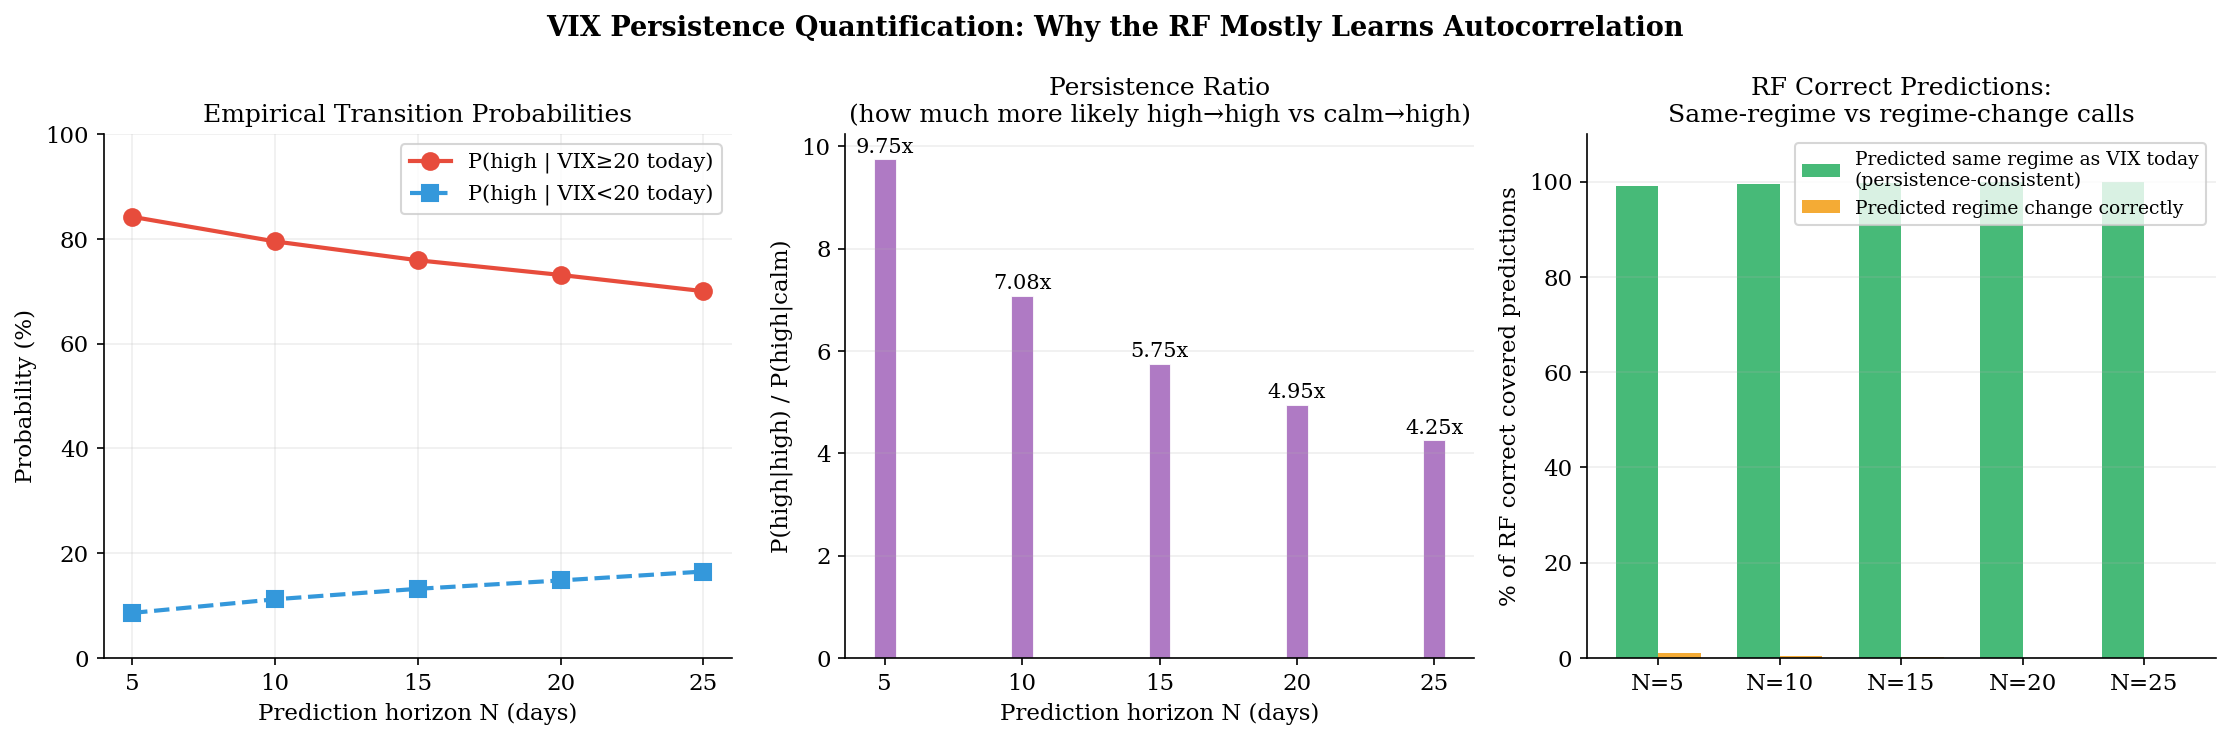
\includegraphics[width=\textwidth]{persistence_quantify.png}
    \caption{Left: empirical transition probabilities conditional on today's regime (all test
    days). Center: persistence ratio P(H$\mid$H)/P(H$\mid$C). Right: decomposition of RF
    correct \emph{covered} predictions into same-regime and regime-change calls. At
    $N \geq 20$, 100\% of correct predictions are same-regime.}
    \label{fig:persist_quant}
\end{figure}

The persistence ratio---the relative probability of a high regime in $N$ days conditional on
today's regime---reaches 9.75$\times$ at $N = 5$, and the same-regime share of the RF's correct
covered predictions rises from 99.0\% at $N = 5$ to 100\% at $N \geq 20$
(Table~\ref{tab:persist_quant}). On the days it chooses to cover, the RF adds no directional
forecasting beyond VIX autocorrelation.

\subsection{Regime Transition Analysis}
\label{sec:transitions}

We classify each test day by the regime at time $t$ and the realized regime at $t + N$, creating
four transition categories: calm$\to$calm, calm$\to$high, high$\to$calm, and high$\to$high.

\begin{table}[H]
\centering
\caption{RF selective coverage and accuracy by regime transition type ($\tau = 0.25$, test
set; accuracy on covered days within each transition type). Calm$\to$high accuracy is
\textbf{0\%} at all horizons: every covered prediction on a day about to spike is a confident
``stay calm'' signal.}
\label{tab:trans}
\begin{tabular}{lcccccc}
\toprule
Transition & \multicolumn{3}{c}{$N = 5$} & \multicolumn{3}{c}{$N = 10$} \\
\cmidrule(lr){2-4}\cmidrule(lr){5-7}
           & Days & Coverage & Acc (covered) & Days & Coverage & Acc (covered) \\
\midrule
calm $\to$ calm & 614 & 87.1\% & 99.6\% & 587 & 71.6\% & 100.0\% \\
calm $\to$ high &  79 & 45.6\% & \textbf{0.0\%}   & 101 & 41.6\% & \textbf{0.0\%} \\
high $\to$ calm &  84 & 35.7\% & 23.3\%            & 111 & 18.0\% & 10.0\% \\
high $\to$ high & 222 & 72.5\% & 99.4\%            & 199 & 59.3\% & 100.0\% \\
\bottomrule
\end{tabular}
\end{table}

\begin{figure}[H]
    \centering
    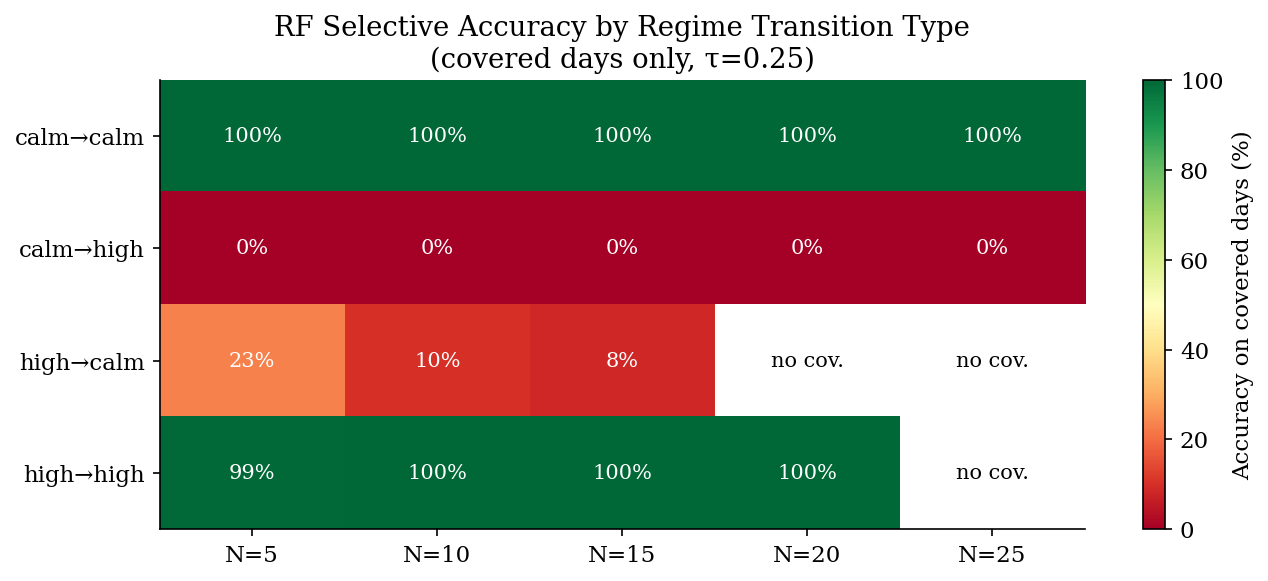
\includegraphics[width=0.65\textwidth]{transition_analysis.png}
    \caption{RF selective accuracy by regime transition type and horizon (covered days only,
    $\tau = 0.25$). Calm$\to$high rows are uniformly 0\% at all horizons.}
    \label{fig:trans}
\end{figure}

At $N = 5$, the model covers 36 of 79 calm$\to$high days (45.6\%). On every single one of those
36 days, it issues a confident ``stay calm'' prediction and is wrong. The mechanism is clear: VIX
comfortably below 20 generates calibrated probabilities below 0.25, triggering a high-confidence
calm prediction.

\paragraph{How many independent events does the 0\% rest on?}
Because transition days cluster around volatility episodes, day counts overstate the number of
independent observations. Grouping the covered calm$\to$high days into episodes (a gap of more
than 10 trading days starts a new episode), the 0\% record at $N = 5$ spans \textbf{16 distinct
episodes} between August 2022 and January 2026---including the August 2022 bear-market rally
failure, the February 2023 repricing, the October 2023 rate scare, the July--August 2024
carry-trade unwind, and the September--October 2025 and January 2026 spikes. The corresponding
counts are 15 episodes at $N = 10$, 12 at $N = 15$, and 4--5 at $N = 20$ and 25. At short
horizons, the transition failure is therefore replicated across a substantial number of
independent market events; at the two longest horizons the episode count is small, and the 0\%
figure there should be read as consistent with low---but not precisely estimated---transition
skill.

\paragraph{Structural caveat.}
This failure is not a model-specific defect: it is an expected structural property of the
prediction problem. Calm$\to$high transitions are disproportionately triggered by exogenous
events---geopolitical shocks, central bank surprises, sudden liquidity dislocations---whose onset
leaves no advance signature in publicly available daily price and macro features. The diagnostic
value of 0\% covered accuracy is that the confidence filter fails to surface its own ignorance,
issuing confident wrong predictions on covered transition days rather than abstaining.

\paragraph{Event case studies.}
Figure~\ref{fig:events} documents the model's behavior during four major volatility events in
the test set: the 2022 bear-market VIX peak (June 2022), the UK gilt crisis (October 2022), the
SVB banking collapse (March 2023), and the Japan carry-trade unwind (August 2024, when VIX
reached 65).

\begin{figure}[H]
    \centering
    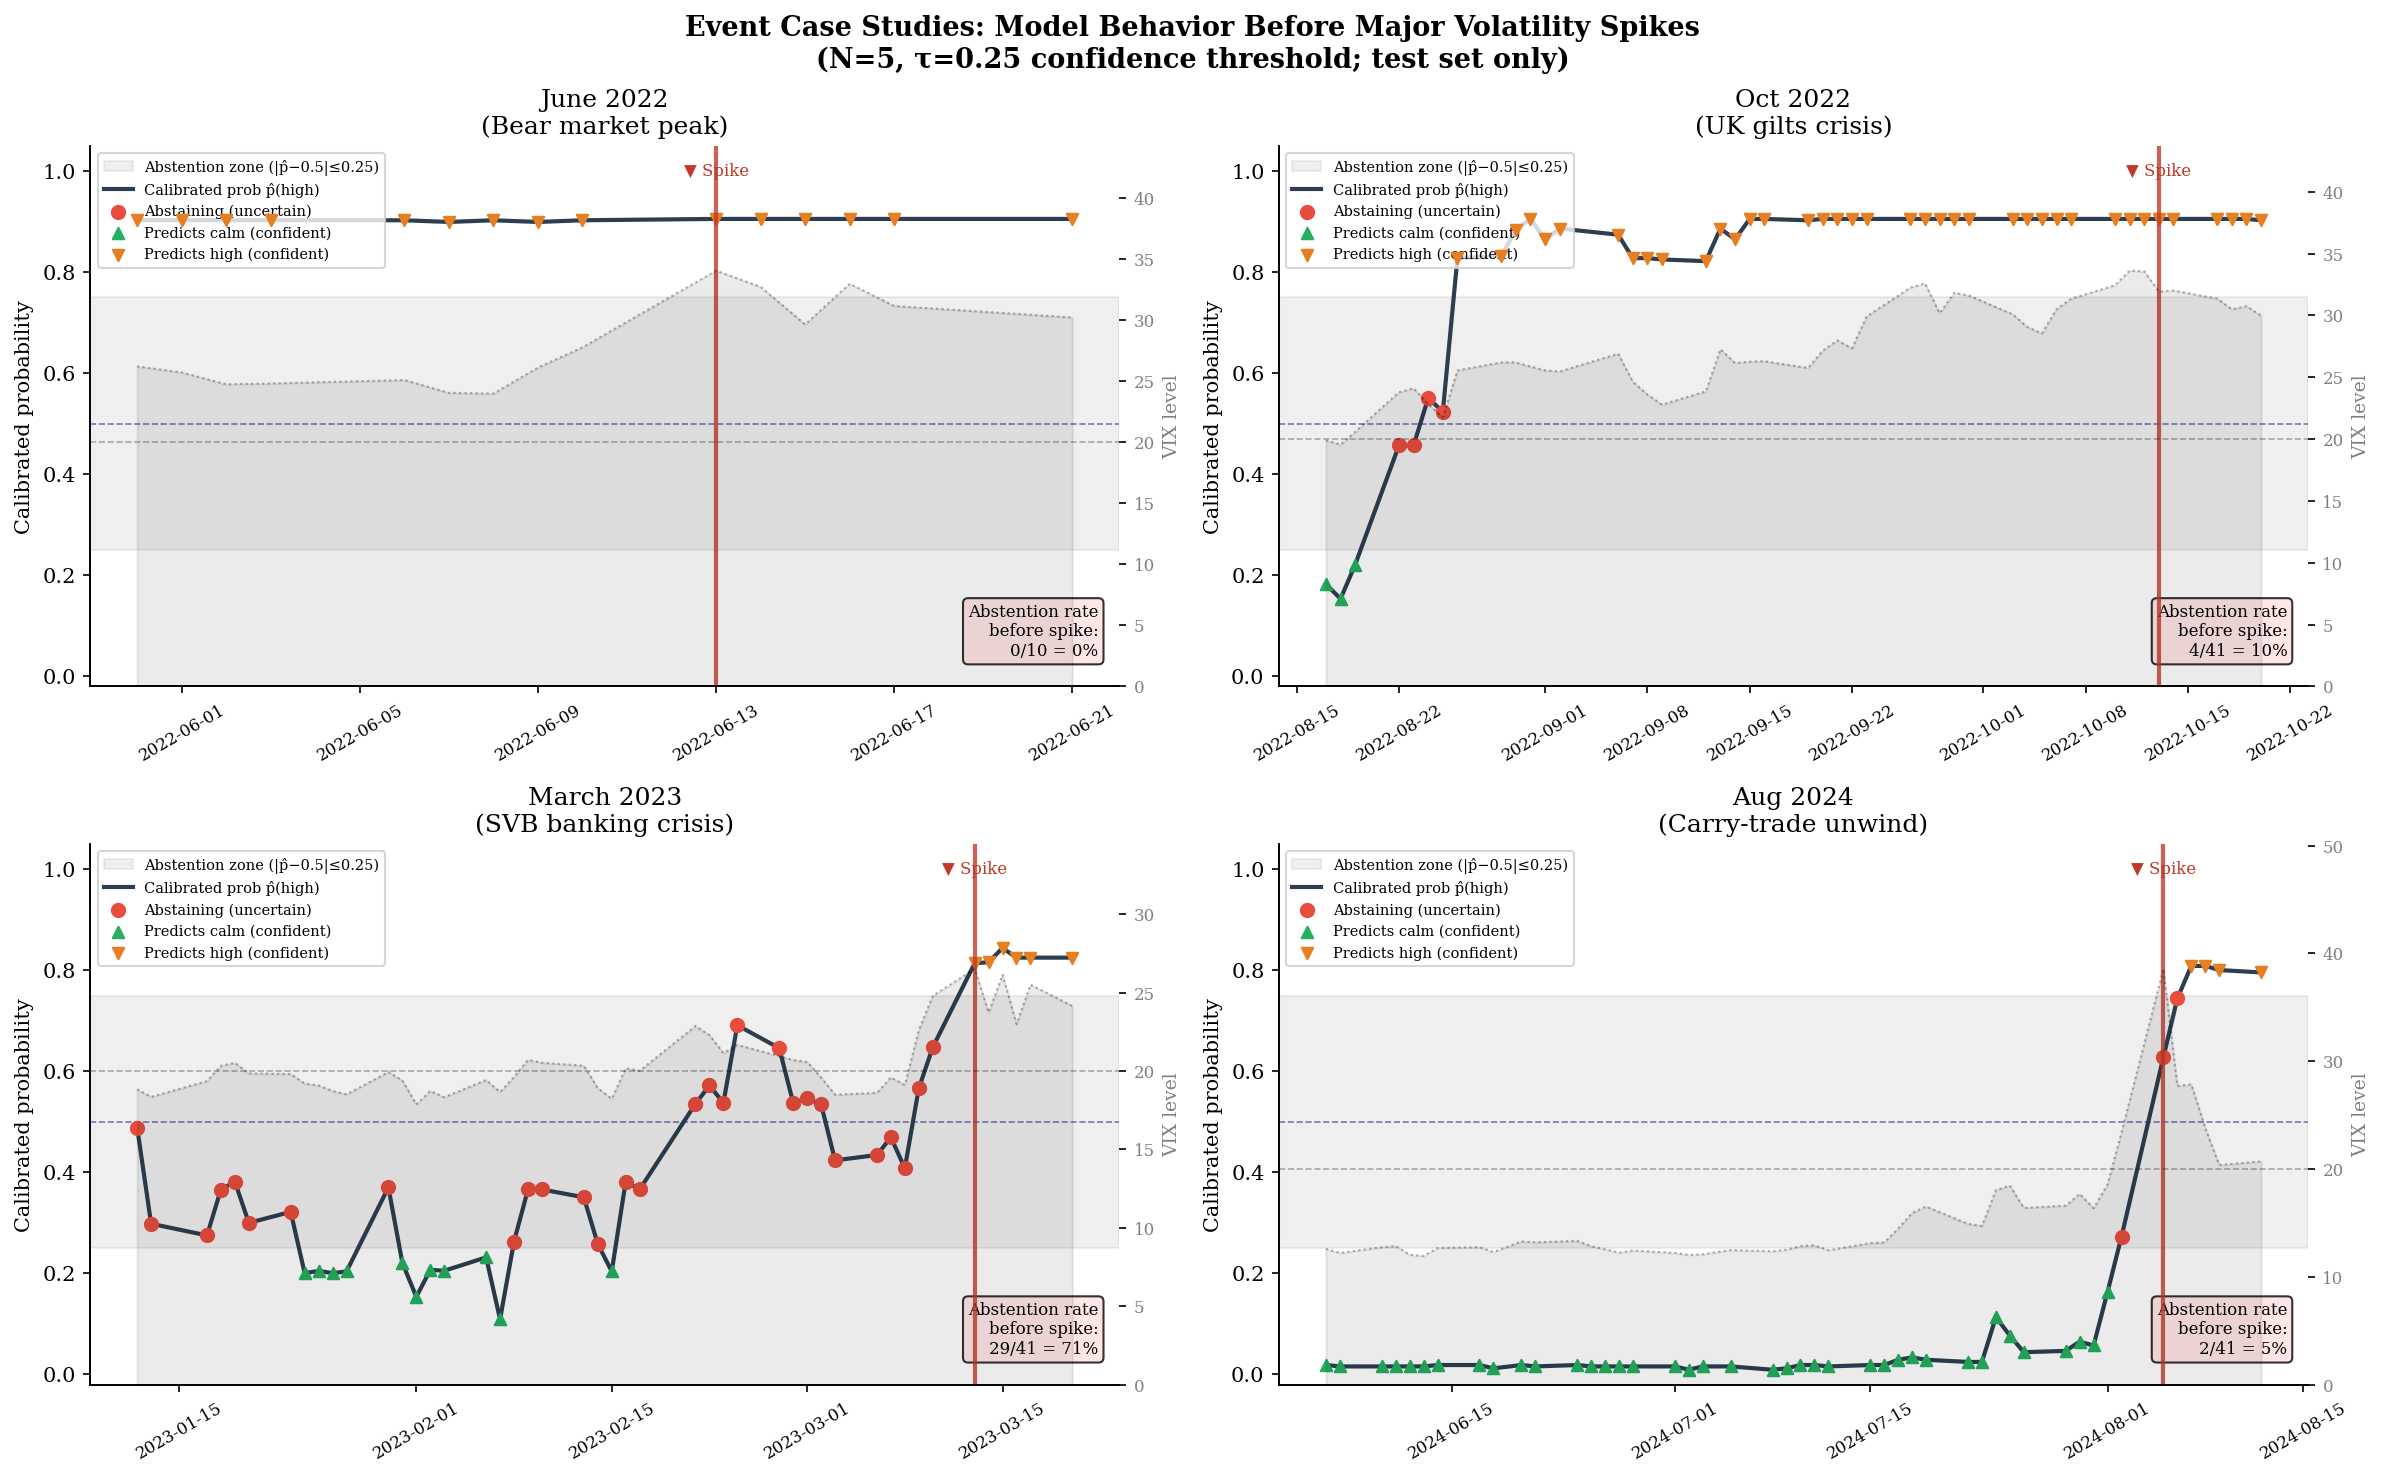
\includegraphics[width=\textwidth]{event_case_studies.png}
    \caption{Model behavior ($\hat{p}_t$, $N = 5$, $\tau = 0.25$) for up to 40 trading days
    before four major volatility events (the June 2022 window is shorter because the test
    period begins in mid-2022). In all four cases the model issues confident calm predictions
    leading up to the event.}
    \label{fig:events}
\end{figure}

Across all four events the pattern is consistent: the model issues confident ``stay calm''
predictions on the days leading up to each spike. The August 2024 carry-trade unwind shows
essentially no anticipatory signal; $\hat{p}_t$ remains below $0.5 - \tau$ until the day the
spike materializes.

\paragraph{Cost-weighting does not rescue calm$\to$high recall.}
To test whether the failure is informational rather than objective-function-driven, we refit the RF
with explicit class weights $\{0{:}1, 1{:}w\}$ for $w \in \{1, 5, 10, 20\}$.

\begin{table}[H]
\centering
\caption{Effect of class-weighting on transition coverage and selective accuracy. Calm$\to$high
accuracy is \textbf{0.0\%} at every weight for both horizons.}
\label{tab:reweight}
\begin{tabular}{ccrrcrc}
\toprule
$N$ & $w$ & C$\to$H Cov & C$\to$H Acc & C$\to$C Cov & C$\to$C Acc & Sel Acc \\
\midrule
5 &  1 & 45.6\% & \textbf{0.0\%} & 87.1\% & 99.6\%  & 91.9\% \\
5 &  5 & 46.8\% & \textbf{0.0\%} & 87.1\% & 100.0\% & 92.2\% \\
5 & 10 & 49.4\% & \textbf{0.0\%} & 87.3\% & 100.0\% & 92.3\% \\
5 & 20 & 48.1\% & \textbf{0.0\%} & 84.4\% & 100.0\% & 91.8\% \\
\midrule
10 &  1 & 41.6\% & \textbf{0.0\%} & 71.6\% & 100.0\% & 90.0\% \\
10 &  5 & 49.5\% & \textbf{0.0\%} & 77.7\% & 100.0\% & 89.5\% \\
10 & 10 & 58.4\% & \textbf{0.0\%} & 80.4\% & 100.0\% & 87.4\% \\
10 & 20 & 57.4\% & \textbf{0.0\%} & 82.8\% & 100.0\% & 87.4\% \\
\bottomrule
\end{tabular}
\end{table}

The failure to predict calm$\to$high transitions is \emph{informational with respect to this
feature set}, not objective-function-driven: no reweighting of the loss surfaces transition
signal that the 36 daily features do not contain. Whether richer information
sets---intraday options flow, news text, macro surprise indices---could anticipate some
transitions remains an open question we return to in the Limitations.

\paragraph{Abstention as a leading indicator.}

\begin{figure}[H]
    \centering
    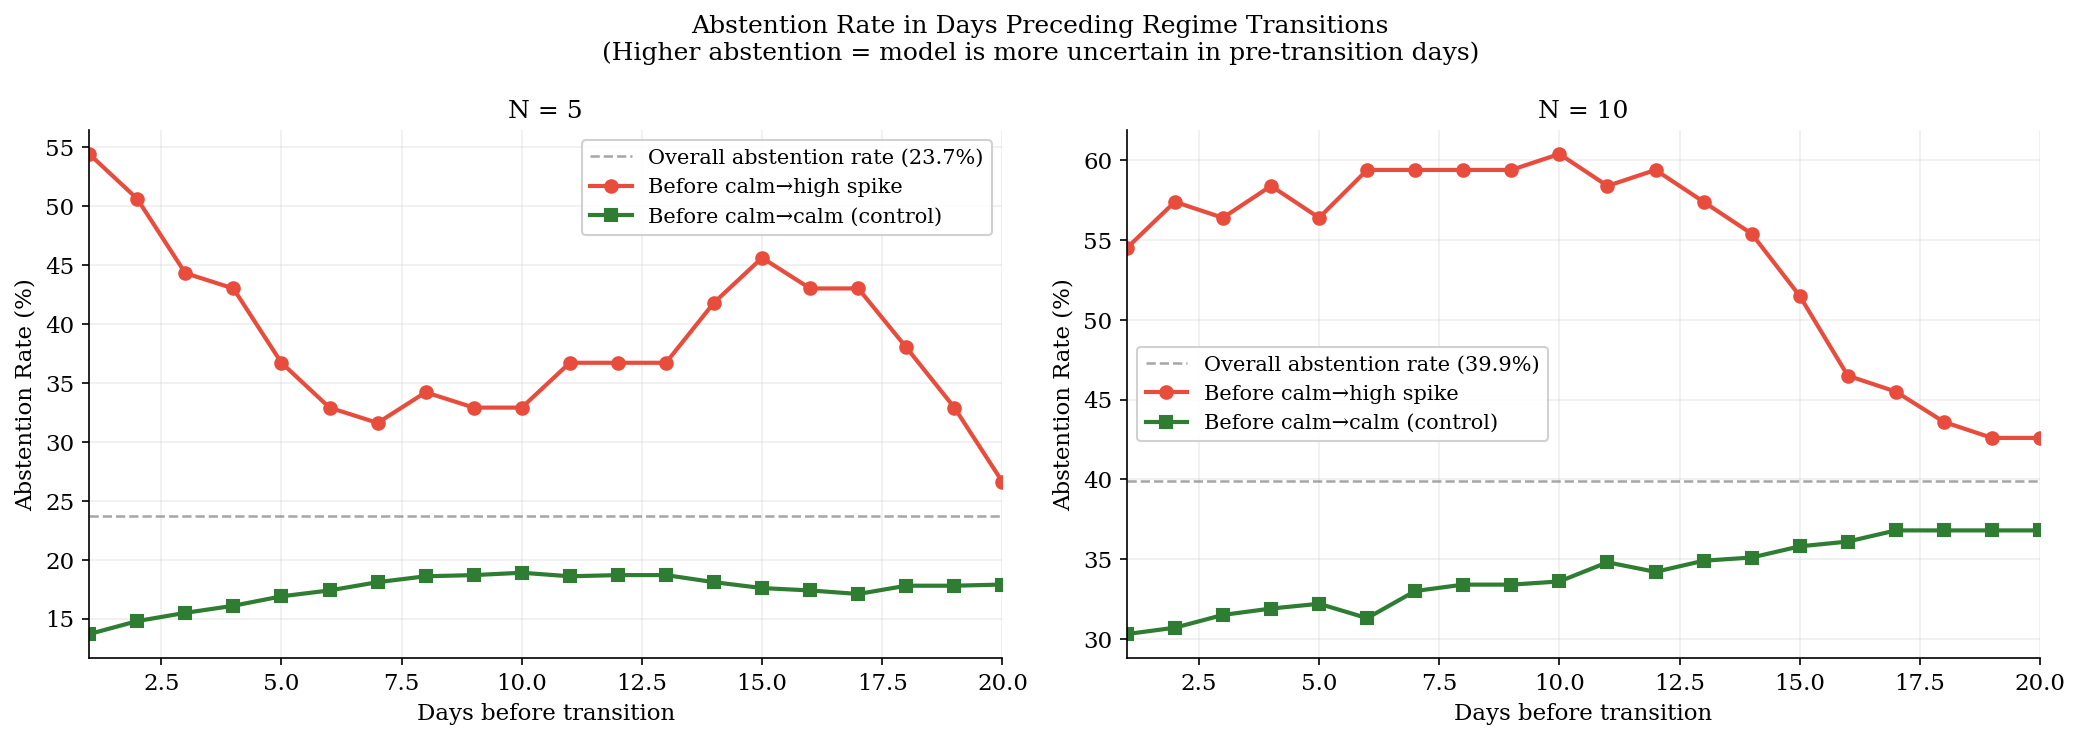
\includegraphics[width=0.85\textwidth]{abstention_analysis.png}
    \caption{Abstention rate (fraction of all test days on which the model declines to
    predict) before calm$\to$high transitions (red) vs.\ calm$\to$calm days (green). At
    lag = 1 day, the abstention rate before spikes is more than double the overall rate.}
    \label{fig:abstention}
\end{figure}

At $N = 5$, the abstention rate immediately before a calm$\to$high transition is 54.4\%,
compared to 13.7\% before calm$\to$calm days and 23.7\% overall---a 2.3$\times$ elevation.
However, a confound test shows that VIX proximity to the threshold (AUC $= 0.805$) explains most
of this signal; the abstention indicator alone achieves AUC $= 0.708$. At $N = 5$, abstention
carries a small residual signal beyond proximity (likelihood-ratio $p = 0.001$ on the evaluation
sample, treated as descriptive rather than confirmatory). This observation should be treated as
hypothesis-generating and requires dedicated out-of-sample confirmation.

\subsection{Walk-Forward Validation}
\label{sec:wf}

\begin{table}[H]
\centering
\caption{5-fold expanding walk-forward validation (fold means $\pm$ std of accuracy on each
fold's covered days; persistence threshold calibrated on each fold's training window). Shaded
rows indicate that at $N = 20$ the RF/HGB standard deviations exceed 25 pp; persistence
remains stable.}
\label{tab:wf}
\begin{tabular}{cccccc}
\toprule
Model & $N$ & Mean Baseline & Std & Mean Selective & Std \\
\midrule
Random Forest    & 5  & 82.8\% & 9.7\%  & 92.2\% & 1.7\%  \\
Persistence      & 5  & 88.0\% & 3.2\%  & \textbf{92.7\%} & 3.6\%  \\
HGB              & 5  & 84.0\% & 8.0\%  & 84.6\% & 9.7\%  \\
\midrule
Random Forest    & 10 & 72.3\% & 22.7\% & 85.9\% & 7.7\%  \\
Persistence      & 10 & 84.8\% & 4.5\%  & \textbf{89.7\%} & 5.0\%  \\
HGB              & 10 & 70.9\% & 22.9\% & 77.3\% & 15.2\% \\
\midrule
\rowcolor[gray]{0.9}
Random Forest    & 20 & 67.5\% & 22.8\% & 67.1\% & 28.3\% \\
Persistence      & 20 & 81.5\% & 3.9\%  & \textbf{84.5\%} & 6.9\%  \\
\rowcolor[gray]{0.9}
HGB              & 20 & 63.6\% & 25.2\% & 61.4\% & 29.9\% \\
\bottomrule
\end{tabular}
\end{table}

Coverage-matched persistence at $N = 5$ achieves 92.7\% $\pm$ 3.6\%---slightly higher mean
than RF (92.2\% $\pm$ 1.7\%). At $N = 10$, persistence (89.7\% $\pm$ 5.0\%) exceeds RF
selective (85.9\% $\pm$ 7.7\%). At $N = 20$, both RF and HGB show standard deviations
exceeding 25 pp across folds, while persistence remains stable at 84.5\% $\pm$ 6.9\%. The
practical reliable prediction window is approximately $N \leq 10$.

\subsection{LSTM Comparison}
\label{sec:lstm}

A two-layer LSTM network is trained on sliding windows of the past 20 trading days of all 36
features, using the same 80/20 chronological split. The LSTM uses hidden size 64, dropout 0.3,
and is trained for 40 epochs with the Adam optimizer. The architecture was chosen as the
standard recurrent sequence baseline in financial ML: two layers and hidden size 64 give
roughly the parameter budget of the tree ensembles, the 20-day window matches the longest
lookback in the engineered feature set (so the LSTM sees the same information horizon), and
dropout 0.3 is a conventional regularization level for series of this length. We did not sweep
architectures or window lengths; the LSTM's role here is not to maximize sequence-model
performance but to test whether temporal memory per se recovers transition signal that the
static ensembles miss. Larger attention-based architectures are a direction for future work,
though the results below suggest the constraint is informational rather than architectural.

\begin{table}[H]
\centering
\caption{LSTM vs.\ RF at $\tau = 0.25$. BalAcc = balanced accuracy on covered days.
Both models are evaluated on the subsample of test days with a complete 20-day feature
window, so the RF columns differ slightly from Table~\ref{tab:main}, which uses all test
days.}
\label{tab:lstm}
\begin{tabular}{cccccc}
\toprule
$N$ & LSTM Sel Acc & LSTM Cov & LSTM BalAcc & RF Sel Acc & RF Cov \\
\midrule
5  & 76.5\% & 87.0\% & 76.0\% & 91.7\% & 77.0\% \\
10 & 71.8\% & 90.7\% & 64.7\% & 89.3\% & 64.3\% \\
\bottomrule
\end{tabular}
\end{table}

The LSTM achieves non-zero calm$\to$high covered accuracy (34.9\% at $N = 5$; 19.1\% at
$N = 10$)---unlike the RF's 0\%---but both figures are substantially below the 50\% random
baseline, meaning the LSTM is wrong more often than right on transition days. Architectural
richness (20-day temporal memory) does not resolve the information constraint: the daily feature
set does not carry the event-anticipation content needed to forecast volatility spikes.

\subsection{SHAP Feature Attribution}
\label{sec:shap}

\begin{figure}[H]
    \centering
    
\includegraphics[width=0.92\textwidth]{shap_analysis.png}
    \caption{Mean absolute SHAP values (top 15 of 36 features) at $N = 5$ (left) and $N = 10$
    (right). VIX technical features account for 71.9\% and 64.7\% of total SHAP mass,
    respectively.}
    \label{fig:shap}
\end{figure}

VIX technical features account for \textbf{71.9\%} of total SHAP mass at $N = 5$ and
\textbf{64.7\%} at $N = 10$. The dominant features are all smoothed or envelope transforms of
the current VIX level. The SHAP decomposition is consistent with the model's predictions being
driven overwhelmingly by VIX autocorrelation, with negligible contribution from the broader
cross-asset and macro feature set. We note the standard caveat that SHAP values measure a
model's attribution of its own predictions, not causal importance \citep{lundberg2017}: the
analysis shows what the fitted model relies on, and cannot rule out that the cross-asset
features carry signal a differently specified model could exploit.

\subsection{Statistical Significance of the Persistence Gap}
\label{sec:bootstrap}

We apply a moving-block bootstrap to the paired accuracy difference (RF selective minus
persistence, with the persistence threshold frozen from the training window). The default block
length is $\max(\sqrt{N_\text{test}},\, 20) \approx 32$ days \citep{kunsch1989}; 2,000
bootstrap replicates are drawn. Because overlapping $N$-day-ahead labels induce serial
dependence of order at least $N$ in the loss differentials---on top of regime persistence that
lasts far longer---we additionally re-run the bootstrap at block lengths of 60 and 90 days
(Appendix~\ref{app:blocklen}).

\begin{table}[H]
\centering
\caption{Moving-block bootstrap 95\% confidence intervals for the RF-minus-persistence
selective accuracy gap (block length 32 days). Only the $N = 10$ interval excludes zero;
this holds at block lengths 60 and 90 as well (Appendix~\ref{app:blocklen}).}
\label{tab:boot}
\begin{tabular}{crrr}
\toprule
$N$ & Gap (pp) & 95\% CI lower & 95\% CI upper \\
\midrule
5  & $+1.70$ & $-0.56$ & $+4.12$ \\
10 & $+2.82$ & $+0.18$ & $+5.27$ \\
15 & $+4.42$ & $-0.47$ & $+9.15$ \\
20 & $+4.15$ & $-3.09$ & $+12.70$ \\
25 & $+7.36$ & $-2.89$ & $+20.71$ \\
\bottomrule
\end{tabular}
\end{table}

Four of five confidence intervals include zero; the exception is $N = 10$, where the RF's
aggregate advantage of $+2.8$ pp is statistically significant. The McNemar test on jointly
covered days clarifies what this aggregate gap does---and does not---consist of. At
$N \in \{10, 20, 25\}$, RF and persistence make \emph{identical} predictions on every jointly
covered day ($b = c = 0$, $p = 1.000$). At $N = 5$ they disagree on 3 of 708 jointly covered
days and at $N = 15$ on 1 of 462 (in the RF's favor; $b = 0$ in every case---persistence never
beats the RF on a shared day---with $p \geq 0.08$ throughout). The significant $N = 10$
aggregate gap therefore arises entirely from \emph{which} days each rule covers: on the days
both systems predict, their predictions coincide exactly. This is coverage-composition
skill---the RF's confidence score is a somewhat better abstention trigger than raw distance to
the threshold---rather than predictive disagreement, and we quantify it directly in
Section~\ref{sec:joint_coverage} and the risk--coverage analysis of
Section~\ref{sec:risk_coverage}. Excluding the 2022 bear-market period (149--165 test days)
leaves all qualitative conclusions unchanged: calm$\to$high covered accuracy remains 0\% at all
horizons.

\subsection{Composition of the Jointly Covered Set}
\label{sec:joint_coverage}

Matching coverage \emph{rates} does not match \emph{which} days are covered. To make the
comparison concrete, Table~\ref{tab:joint} reports the size of the jointly covered set (days on
which both the RF and the persistence rule predict) and its composition by transition type.

\begin{table}[H]
\centering
\caption{Size and transition-type composition of the jointly covered set
(RF $\cap$ persistence, $\tau = 0.25$). Percentages in the four rightmost columns are shares
of the joint set.}
\label{tab:joint}
\resizebox{\textwidth}{!}{%
\begin{tabular}{cccccccc}
\toprule
$N$ & Joint days & \% of test & RF cov & calm$\to$calm & calm$\to$high & high$\to$calm & high$\to$high \\
\midrule
5  & 708 & 70.9\% & 76.3\% & 70.9\% & 4.0\% & 3.1\% & 22.0\% \\
10 & 556 & 55.7\% & 60.1\% & 70.3\% & 5.8\% & 3.1\% & 20.9\% \\
15 & 462 & 46.3\% & 51.3\% & 70.6\% & 6.1\% & 2.6\% & 20.8\% \\
20 & 257 & 25.8\% & 31.7\% & 83.3\% & 4.3\% & 0.0\% & 12.5\% \\
25 & 113 & 11.4\% & 26.9\% & 92.9\% & 7.1\% & 0.0\% & 0.0\% \\
\bottomrule
\end{tabular}}
\end{table}

The joint set is dominated by regime-stable days: 92.9\% at $N = 5$ (calm$\to$calm plus
high$\to$high) rising to 92.9\% calm$\to$calm alone at $N = 25$, where not a single
high$\to$calm or high$\to$high day survives both filters. We state the implication plainly:
the $b = c = 0$ result is close to guaranteed \emph{given} the composition of the joint
set---deep-calm and deep-high days on which any reasonable rule agrees. That is not a
weakness of the analysis; it is the finding. The confidence filter and the
distance-to-threshold rule select nearly the same easy days, which is precisely why selective
accuracy is not evidence of skill beyond persistence on this task.

\subsection{Risk--Coverage Analysis}
\label{sec:risk_coverage}

Nearly all results above are reported at $\tau = 0.25$. Following standard practice in the
selective prediction literature \citep{geifman2019}, Figure~\ref{fig:risk_coverage} reports
full risk--coverage curves---selective error as a function of coverage, swept over the entire
confidence range---for RF, HGB, XGBoost, and the persistence rule (whose confidence score is
distance to the threshold, $|\text{VIX}_t - 20|$), with the area under the risk--coverage
curve (AURC) in Table~\ref{tab:aurc}.

\begin{figure}[H]
    \centering
    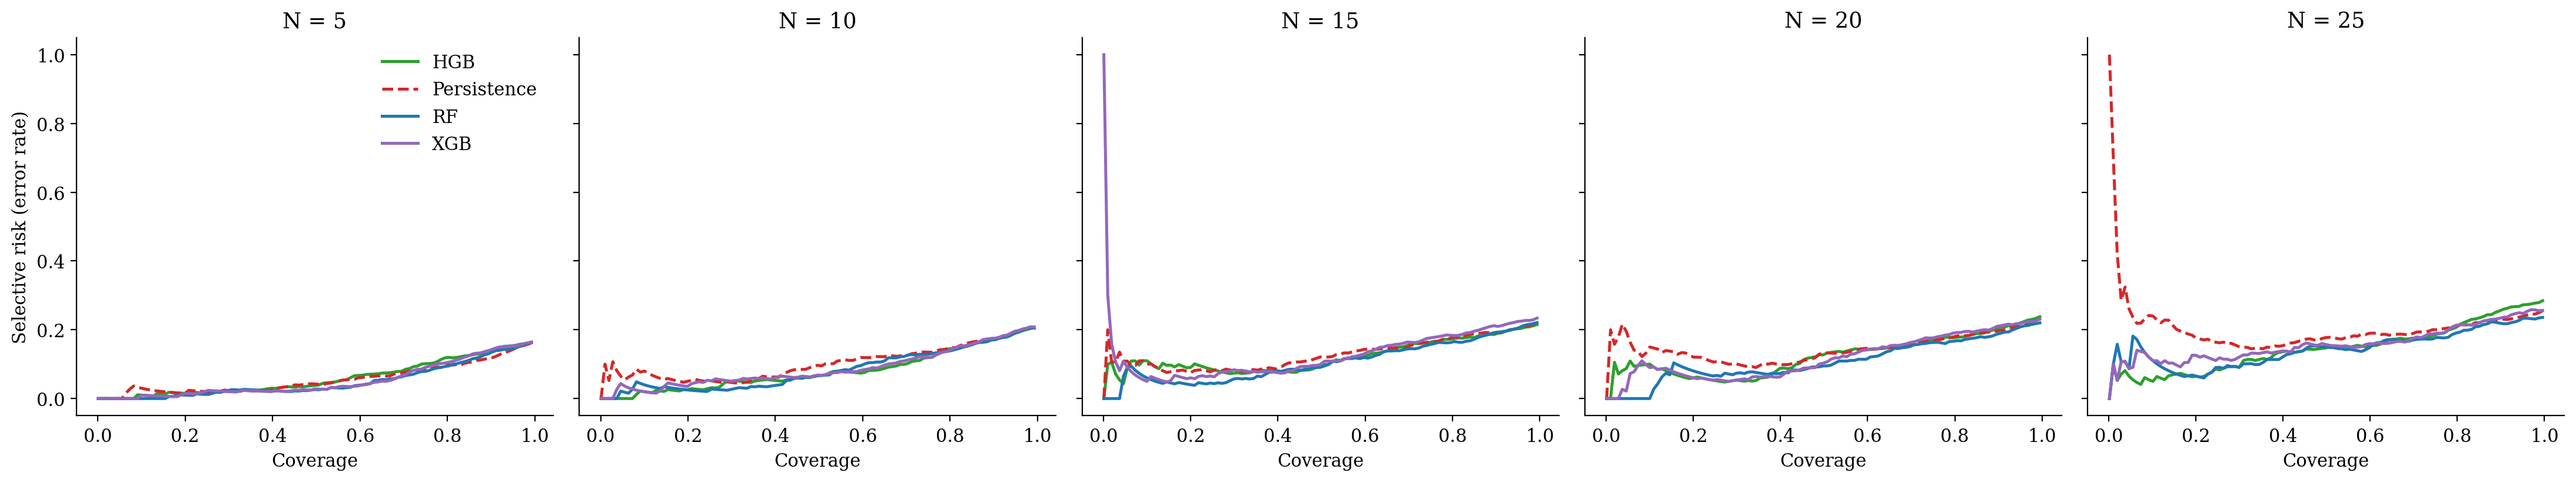
\includegraphics[width=\textwidth]{risk_coverage.png}
    \caption{Risk--coverage curves per horizon (test set; selective risk = error rate on
    covered days as coverage varies over the full confidence sweep). Persistence uses
    $|\text{VIX}_t - 20|$ as its confidence score.}
    \label{fig:risk_coverage}
\end{figure}

\begin{table}[H]
\centering
\caption{Area under the risk--coverage curve (AURC; lower is better) by model and horizon.}
\label{tab:aurc}
\begin{tabular}{ccccc}
\toprule
$N$ & RF & HGB & XGBoost & Persistence \\
\midrule
5  & \textbf{0.049} & 0.060 & 0.053 & 0.056 \\
10 & 0.083 & \textbf{0.081} & 0.087 & 0.104 \\
15 & \textbf{0.107} & 0.123 & 0.130 & 0.130 \\
20 & \textbf{0.109} & 0.124 & 0.120 & 0.146 \\
25 & \textbf{0.146} & 0.147 & 0.161 & 0.206 \\
\bottomrule
\end{tabular}
\end{table}

The threshold-free view adds an honest nuance to the persistence story. The RF attains the
lowest AURC at four of five horizons, and all three ML models rank their own confidence better
than the distance-to-threshold heuristic over the full coverage range---the ML confidence
ordering is genuinely more informative about which days are easy. However, this ranking
advantage operates almost entirely within the regime-stable population: as
Section~\ref{sec:joint_coverage} shows, at deployed coverage rates the covered sets nearly
coincide, and as Section~\ref{sec:transitions} shows, no confidence ordering surfaces
calm$\to$high days as predictable. Better ranking of easy days does not translate into
detection of the transitions that matter for risk management.

\subsection{Cost-Weighted Utility Analysis}
\label{sec:utility}

\begin{equation}
    U = -\frac{\text{FP} + C \cdot \text{FN}}{n_{\text{predictions}}}
    \label{eq:utility}
\end{equation}

\begin{table}[H]
\centering
\caption{Cost-weighted utility per prediction under different FN/FP cost ratios $C$. Higher
utility (closer to 0) is better. Bolded entries show where persistence dominates RF selective.}
\label{tab:utility}
\begin{tabular}{ccrrrr}
\toprule
$N$ & $C$ & RF Selective & Persistence & RF Baseline & Always Calm \\
\midrule
5 &  1 & $-0.081$ & $-0.087$ & $-0.166$ & $-0.301$ \\
5 &  5 & $-0.276$ & $-0.286$ & $-0.515$ & $-1.507$ \\
5 & 10 & $-0.518$ & $-0.535$ & $-0.950$ & $-3.013$ \\
5 & 20 & $-1.004$ & $-1.033$ & $-1.821$ & $-6.026$ \\
\midrule
10 &  1 & $-0.100$ & $-0.120$ & $-0.205$ & $-0.301$ \\
10 &  5 & $-0.380$ & $\mathbf{-0.326}$ & $-0.626$ & $-1.503$ \\
10 & 10 & $-0.730$ & $\mathbf{-0.584}$ & $-1.152$ & $-3.006$ \\
10 & 20 & $-1.430$ & $\mathbf{-1.100}$ & $-2.204$ & $-6.012$ \\
\bottomrule
\end{tabular}
\end{table}

At $N = 10$, persistence at matched coverage dominates RF selective prediction under any moderate
false-negative cost asymmetry ($C \geq 5$). The RF selective framework is utility-beneficial only
when false positives are as costly as false negatives ($C = 1$).

% -----------------------------------------------------------------------
\section{Replication: S\&P 500 Trend-Regime Classification}
\label{sec:replication}
% -----------------------------------------------------------------------

To test whether the persistence illusion is specific to volatility forecasting, we replicate the
full diagnostic protocol on S\&P 500 trend-regime classification using the same feature set and
model specification. The label is:
\begin{equation}
    \text{BEAR}_{N,t} = \begin{cases} 1 & \text{if } \text{SP500}_{t+N} < \overline{\text{SP500}}_{200,t+N} \\ 0 & \text{otherwise} \end{cases}
\end{equation}

The persistence baseline here predicts the current trend regime continues, with abstention
when the S\&P 500 is within a band of its 200-day moving average; the band is measured as a
\emph{fraction} of the moving average (so it is scale-free across the 2006--2026 index range)
and is calibrated on the training window to match the RF's training coverage, then frozen.

\begin{table}[H]
\centering
\caption{S\&P 500 trend-regime replication (persistence band calibrated on training window).
Accuracies on each system's covered test days. RF$-$Persist is negative at four of five
horizons: persistence matches or dominates the RF selective classifier.}
\label{tab:sp500}
\begin{tabular}{cccccccc}
\toprule
$N$ & Base rate & RF Cov & Persist Cov & Persistence & HAR-analog & RF Sel & RF$-$Persist \\
\midrule
5  & 22.0\% & 74.4\% & 91.5\% & \textbf{97.9\%} & 78.0\% & 96.0\% & $-2.0$ pp \\
10 & 21.9\% & 68.3\% & 90.8\% & 94.7\%          & 78.1\% & 94.9\% & $+0.2$ pp \\
15 & 21.9\% & 69.7\% & 91.1\% & \textbf{92.8\%} & 78.1\% & 90.9\% & $-1.9$ pp \\
20 & 21.8\% & 70.3\% & 91.4\% & \textbf{90.5\%} & 78.2\% & 87.7\% & $-2.8$ pp \\
25 & 21.7\% & 59.5\% & 89.5\% & \textbf{89.8\%} & 78.3\% & 88.3\% & $-1.4$ pp \\
\bottomrule
\end{tabular}
\end{table}

\begin{table}[H]
\centering
\caption{S\&P 500 transition accuracy. Bull$\to$bear covered accuracy is \textbf{0\%}---exact
mirror of VIX calm$\to$high.}
\label{tab:sp500_trans}
\begin{tabular}{cccccc}
\toprule
$N$ & Transition & Days & Coverage & Acc (covered) & Same-regime \% \\
\midrule
5  & bull$\to$bull &  749 & 88.8\% & 100.0\% & 99.2\% \\
5  & bull$\to$bear &   25 & 68.0\% & \textbf{0.0\%} & \\
\midrule
10 & bull$\to$bull &  730 & 86.2\% & 100.0\% & 98.6\% \\
10 & bull$\to$bear &   39 & 71.8\% & \textbf{0.0\%} & \\
\bottomrule
\end{tabular}
\end{table}

\begin{figure}[H]
    \centering
    
\includegraphics[width=\textwidth]{sp500_replication.png}
    \caption{S\&P 500 trend-regime replication (covered test days; persistence band frozen from
    the training window). Left: RF vs.\ persistence selective accuracy---persistence matches or
    dominates at four of five horizons. Center: persistence ratio of 23.8$\times$ at $N = 5$.
    Right: bull$\to$bear covered accuracy is 0\%, replicating the VIX calm$\to$high finding.}
    \label{fig:sp500}
\end{figure}

The persistence ratio is \textbf{23.8$\times$} at $N = 5$---more than twice the VIX ratio of
9.75$\times$---and persistence matches or beats the RF at four of five horizons (RF$-$Persist:
$-1.4$ to $-2.8$ pp, with a $+0.2$ pp tie at $N = 10$). Note that the frozen persistence band
covers \emph{more} of the test window than the RF (roughly 90\% vs.\ 60--74\%), so its
advantage is not an artifact of retreating to an easier covered subset: persistence predicts
on more days, including harder ones, and still matches or exceeds the RF. Bull$\to$bear covered accuracy is
\textbf{0.0\%} at both $N = 5$ and $N = 10$, replicating the VIX calm$\to$high finding exactly,
and RF balanced accuracy again degrades toward 50\% as the horizon grows. The replication is
consistent with the persistence illusion being a structural consequence of applying selective
prediction to highly autocorrelated binary time series rather than a VIX-specific artifact,
though we emphasize that two markets constitute supporting evidence for that broader
hypothesis, not a demonstration of it.

% -----------------------------------------------------------------------
\section{Conclusions}
\label{sec:conclusion}
% -----------------------------------------------------------------------

The primary contribution of this paper is a six-component diagnostic protocol for evaluating
selective prediction systems on serially correlated labels, demonstrated in detail on VIX
regime classification. Applied to this task, the protocol indicates that headline selective
accuracy of 90--94\% largely reflects label persistence rather than multi-feature machine
learning skill. The evidence divides into two tiers, which we state separately.

\textbf{Statistically supported findings.} On jointly covered days, RF and a
training-calibrated persistence rule make identical predictions at $N \in \{10, 20, 25\}$
(McNemar $b = c = 0$) and disagree on at most 3 of 708 shared days at the remaining horizons,
with persistence never winning a disagreement. The moving-block bootstrap on the
RF-minus-persistence gap includes zero at four of five horizons (robust to block lengths of
32--90 days); the one significant gap ($N = 10$, $+2.8$ pp) is attributable to coverage
composition, since predictions on shared days coincide exactly. The HAR-minus-RF bootstrap CIs
include zero at both audited horizons. The confidence filter achieved 0\% covered accuracy on
calm$\to$high transitions at every horizon, across 16 independent transition episodes at
$N = 5$---for RF, HGB, XGBoost, and a forecast-then-threshold HAR model, with an LSTM
performing below chance on the same days---and explicit cost-weighting up to $20{\times}$
did not change this.

\textbf{Descriptive observations.} Point-estimate patterns---the HAR-LR exceeding the RF at
$N = 25$, the ordering among baselines within overlapping confidence intervals, and the
1--7 pp spreads in Table~\ref{tab:baselines}---are reported as descriptive and should not be
read as confirmed effects. We note that many comparisons are performed across horizons and
analyses; because the paper's central claims are \emph{negative} results (absence of
significant gaps), multiplicity concerns cut against finding spurious significance rather than
in favor of our conclusions, but the descriptive tier should be interpreted accordingly.

The scope of the evidence is two highly persistent financial classification problems: VIX
regimes and S\&P 500 trend regimes. The proposition that the persistence illusion afflicts
selective prediction on autocorrelated labels generally is a hypothesis these two cases
support, not a demonstrated property; additional domains are needed before broader claims can
be made.

\subsection*{Practical Implications: Who Should Use This Protocol, and How}
\label{sec:practical}

The protocol is designed for four audiences. \emph{Model validators and model risk management
teams} evaluating internal or vendor regime-classification signals can apply it to determine
whether a marketed accuracy figure survives persistence-matched comparison. \emph{Quantitative
researchers} developing selective classifiers on financial time series can use it to locate
where their model's accuracy comes from before claiming skill. \emph{Referees and editors}
reviewing selective-prediction papers on autocorrelated data can use it as a review checklist.
\emph{Practitioners} deciding whether to deploy a regime signal can use the transition-level
decomposition to see whether the signal works on the days that drive hedging value.

Concretely, we recommend that any selective prediction system on serially correlated labels
report: (i)~balanced accuracy alongside selective accuracy; (ii)~a persistence baseline whose
abstention threshold is calibrated on training data only; (iii)~the size and transition-type
composition of the jointly covered set; (iv)~transition-conditional coverage and accuracy;
(v)~risk--coverage curves and AURC rather than a single threshold; and (vi)~attribution
analysis identifying reliance on autocorrelation proxies. Absence of these six items leaves
open the possibility that reported accuracy is composition-driven.

Selective prediction itself is not the villain of this analysis, and from a risk-management
perspective there remain concrete situations where it adds value despite its inability to
detect transitions. First, \emph{abstention as an uncertainty signal}: the abstention rate
itself carries modest leading-indicator content (rising to 54\% immediately before
calm$\to$high transitions at $N = 5$ in our sample), so a desk can treat a spike in
abstentions---rather than the model's directional calls---as a trigger to review hedges,
tighten position limits, or scale down volatility-sensitive exposure. Used this way, the
system's silence is the signal, and its silence is honest even when its predictions are not
informative. Second, \emph{regime-stable confirmation}: 99--100\% covered accuracy on
regime-stable days is genuinely useful for strategies whose main risk is acting on false
alarms---for example, gating a systematic carry or volatility-selling program that should
stay deployed in confirmed calm regimes and needs protection mainly against spurious exit
signals. Third, \emph{avoiding forced low-confidence calls}: in workflows where a model
output feeds an automated decision, an abstention that routes the day to a human or to a
conservative default is preferable to a forced coin-flip prediction. In each case the
deployment principle is the same: use the selective system for what the diagnostic shows it
can do (confirm continuation, flag its own uncertainty), and refuse to lean on it for what
it cannot (anticipate spikes). What the protocol guards against is mistaking the accuracy of
the covered subset for forecasting skill.

\subsection*{Limitations}

The feature set consists of publicly available daily market data; the transition failure
documented here is a statement about \emph{this information set}, not about all possible
information sets. Two of the feature groups (the CBOE SKEW index and the VIX term-structure
spread) are themselves option-implied, so the negative result already covers the most
accessible option-implied measures; richer sources---intraday options flow, macroeconomic
surprise indices, news sentiment, textual and order-flow data---could in principle anticipate
some exogenous transitions and are the primary open direction. Calm$\to$high transitions are
disproportionately triggered by exogenous shocks---geopolitical events, policy surprises,
sudden liquidity crises---that leave no advance signature in daily price features. The
four-year test period ($\approx$1,000 trading days) is underpowered for distinguishing
accuracy differences of 1--3 pp under serial dependence, and contains 4--16 independent
calm$\to$high episodes depending on horizon. The replication spans two U.S.\ equity-linked
markets; non-U.S.\ volatility indices (e.g., VSTOXX) and other asset classes remain untested.

\subsection*{Future Work}

The primary open direction is feature enrichment: incorporating event-anticipation content such
as options flow dynamics, credit spreads, news-based sentiment, or order-flow imbalance, to
test whether the transition failure reflects the daily public information set or a deeper
unpredictability of exogenous shocks. A two-stage system using the abstention rate as a leading
indicator followed by a conditional spike-prediction model is a second natural direction. Third,
the diagnostic protocol should be applied to additional autocorrelated regime classification
tasks---credit spread regimes, recession prediction, currency crisis indicators---to
characterize how the persistence ratio relates to the severity of the selective-prediction
bias and to test the generality of the persistence-illusion hypothesis.

% -----------------------------------------------------------------------
% REQUIRED STATEMENTS
% -----------------------------------------------------------------------

\section*{Author Contributions}

Conceptualization, A.G.; methodology, A.G.; software, A.G.; formal analysis, A.G.; data
curation, A.G.; investigation, A.G.; writing---original draft, A.G.; writing---review and
editing, J.L.; visualization, A.G.; supervision, J.L. All authors have read and agreed to the
published version of the manuscript.

\section*{Funding}

This research received no external funding.

\section*{Data Availability Statement}

The data used in this study are publicly available. VIX, VIX3M, S\&P 500, gold, Treasury yield,
DXY, and SKEW data are available from Yahoo Finance (\url{https://finance.yahoo.com}).
Macroeconomic data (Federal Funds Rate and yield curve spread) are available from the Federal
Reserve Economic Data (FRED) API (\url{https://fred.stlouisfed.org}). The complete analysis
pipeline---data download, feature engineering, model training, calibration, all baselines,
bootstrap inference, and figure generation---is publicly available at
\url{https://github.com/akshatg10104/VIX_research}.

\section*{Conflicts of Interest}

The authors declare no conflicts of interest.

\section*{Declaration of Generative AI Use}

During the preparation of this work, the authors used Claude (Anthropic) to assist with
analysis-code development, data processing, manuscript drafting, and revision. The study
design, research questions, and interpretation of results are the authors' own; the authors
reviewed, verified, and edited all generated code and text, independently checked the reported
numerical results, and take full responsibility for the content of the published article.

% -----------------------------------------------------------------------
\appendix
\section{Complete Feature List}
\label{app:features}

\begin{table}[H]
\centering
\caption{All 36 engineered features, grouped by category. All features are computed from
information available at or before prediction date $t$.}
\label{tab:features}
\footnotesize
\renewcommand{\arraystretch}{0.95}
\begin{tabular}{llll}
\toprule
\# & Feature name & Definition & Category \\
\midrule
1  & VIX\_SMA10        & 10-day simple moving average of VIX                        & VIX trend \\
2  & VIX\_SMA20        & 20-day simple moving average of VIX                        & VIX trend \\
3  & VIX\_MOM10        & VIX$_t$ $-$ VIX$_{t-10}$                                  & VIX momentum \\
4  & VIX\_MOM20        & VIX$_t$ $-$ VIX$_{t-20}$                                  & VIX momentum \\
5  & VIX\_ROC10        & $({\rm VIX}_t / {\rm VIX}_{t-10}) - 1$                     & VIX momentum \\
6  & VIX\_ROC20        & $({\rm VIX}_t / {\rm VIX}_{t-20}) - 1$                     & VIX momentum \\
7  & VIX\_BB\_STD      & 20-day rolling std.\ of VIX                                & VIX Bollinger \\
8  & VIX\_BB\_UPPER    & VIX\_SMA20 $+$ 2$\times$VIX\_BB\_STD                       & VIX Bollinger \\
9  & VIX\_BB\_LOWER    & VIX\_SMA20 $-$ 2$\times$VIX\_BB\_STD                       & VIX Bollinger \\
10 & VIX\_BB\_POSITION & (VIX$_t$ $-$ VIX\_BB\_LOWER) / (4$\times$VIX\_BB\_STD)    & VIX Bollinger \\
11 & VIX\_RSI14        & 14-day Relative Strength Index of VIX                      & VIX oscillator \\
12 & VIX\_MA\_CROSS      & VIX\_SMA10 $-$ VIX\_SMA20                                  & VIX trend \\
13 & VIX\_TERM\_SPREAD & VIX3M$_t$ $-$ VIX$_t$                                      & VIX structure \\
\midrule
14 & SKEW\_LEVEL       & Raw CBOE SKEW index value                                  & Tail risk \\
15 & SKEW\_CHANGE5        & SKEW$_t$ $-$ SKEW$_{t-5}$                                  & Tail risk \\
16 & SKEW\_CHANGE20       & SKEW$_t$ $-$ SKEW$_{t-20}$                                 & Tail risk \\
\midrule
17 & SP500\_RET1       & Log return of S\&P 500 over 1 day                          & Equity \\
18 & SP500\_RET5       & Log return of S\&P 500 over 5 days                         & Equity \\
19 & SP500\_RET20      & Log return of S\&P 500 over 20 days                        & Equity \\
20 & SP500\_MOM10      & S\&P 500 price at $t$ $-$ price at $t-10$                  & Equity \\
21 & SP500\_MOM20      & S\&P 500 price at $t$ $-$ price at $t-20$                  & Equity \\
22 & SP500\_RVOL       & 20-day realized volatility of S\&P 500 daily returns        & Equity \\
23 & SP500\_DRAWDOWN   & 252-day maximum drawdown of S\&P 500                       & Equity \\
\midrule
24 & GOLD\_RET1        & Log return of gold futures over 1 day                      & Cross-asset \\
25 & GOLD\_RET5        & Log return of gold futures over 5 days                     & Cross-asset \\
26 & GOLD\_RET20       & Log return of gold futures over 20 days                    & Cross-asset \\
27 & TNY\_CHANGE1         & 10Y Treasury yield change over 1 day                       & Cross-asset \\
28 & TNY\_CHANGE5         & 10Y Treasury yield change over 5 days                      & Cross-asset \\
29 & TNY\_CHANGE20        & 10Y Treasury yield change over 20 days                     & Cross-asset \\
30 & DXY\_RET1         & Log return of DXY over 1 day                               & Cross-asset \\
31 & DXY\_RET5         & Log return of DXY over 5 days                              & Cross-asset \\
32 & DXY\_RET20        & Log return of DXY over 20 days                             & Cross-asset \\
\midrule
33 & FEDFUNDS\_CHANGE1M   & Federal Funds Rate change over $\approx$21 trading days    & Macro \\
34 & FEDFUNDS\_CHANGE3M   & Federal Funds Rate change over $\approx$63 trading days    & Macro \\
35 & YIELD\_CURVE\_CHANGE1M & T10Y2Y spread change over $\approx$21 trading days      & Macro \\
36 & YIELD\_CURVE\_CHANGE3M & T10Y2Y spread change over $\approx$63 trading days      & Macro \\
\bottomrule
\end{tabular}
\end{table}

\section{Additional Robustness Results}
\label{app:robustness}

This appendix collects secondary robustness tables referenced in the main text: confidence
threshold sensitivity, VIX regime-threshold robustness (18/20/22), and sustained regime
labels.

\subsection{Threshold Sensitivity}

\begin{table}[H]
\centering
\caption{Random Forest selective accuracy (covered days) and coverage as a function of
confidence threshold $\tau$.}
\label{tab:threshold}
\begin{tabular}{ccccc}
\toprule
$\tau$ & RF $N{=}5$ Acc & $N{=}5$ Cov & RF $N{=}10$ Acc & $N{=}10$ Cov \\
\midrule
0.10 & 86.5\% & 91.0\% & 83.3\% & 90.5\% \\
0.15 & 88.3\% & 85.1\% & 84.7\% & 85.9\% \\
0.20 & 89.0\% & 82.9\% & 86.6\% & 78.5\% \\
0.25 & 91.9\% & 76.3\% & 90.0\% & 60.1\% \\
0.30 & 92.3\% & 73.6\% & 91.8\% & 53.6\% \\
0.35 & 95.0\% & 67.1\% & 95.1\% & 36.5\% \\
0.40 & 97.4\% & 49.0\% & 97.4\% & 15.3\% \\
\bottomrule
\end{tabular}
\end{table}

Accuracy increases monotonically with $\tau$ across all horizons, consistent with the
calibrated probability being a reliable ranking signal. However, as Section~\ref{sec:transitions} shows,
increasing $\tau$ does not improve coverage of transition days---it makes confident wrong
predictions on calm$\to$high days even more selective.

\subsection{Robustness Across VIX Thresholds}

\begin{table}[H]
\centering
\caption{Random Forest accuracy gain (selective accuracy on covered days vs.\ baseline
accuracy on all days) by VIX regime threshold at $\tau = 0.25$.}
\label{tab:robust}
\begin{tabular}{cccc}
\toprule
$N$ & VIX $\geq$ 18 & VIX $\geq$ 20 & VIX $\geq$ 22 \\
\midrule
5  & $+$5.4 pp  & $+$8.5 pp  & $+$7.5 pp  \\
10 & $+$11.3 pp & $+$10.5 pp & $+$10.3 pp \\
15 & $+$14.8 pp & $+$13.8 pp & $+$7.9 pp  \\
20 & $+$22.3 pp & $+$15.9 pp & $+$9.1 pp  \\
25 & $-$14.8 pp & $+$16.9 pp & $+$8.3 pp  \\
\bottomrule
\end{tabular}
\end{table}

The advantage of selective prediction holds across VIX thresholds of 18, 20, and 22 at
$N \leq 20$. The exception is RF at $N = 25$, VIX $\geq$ 18, which shows a gain of $-14.8$ pp,
consistent with the degenerate behavior documented in Table~\ref{tab:extended}.

\subsection{Sustained Regime Labels}
\label{sec:sustained}

\begin{table}[H]
\centering
\caption{Random Forest selective accuracy (covered days) for instantaneous and sustained
regime labels at $\tau = 0.25$.}
\label{tab:sustained}
\begin{tabular}{ccc}
\toprule
$N$ & Instantaneous & Sustained \\
\midrule
5  & 91.9\% & 94.0\% \\
10 & 90.0\% & 93.8\% \\
15 & 90.0\% & 93.8\% \\
20 & 92.7\% & 94.3\% \\
25 & 90.3\% & 89.9\% \\
\bottomrule
\end{tabular}
\end{table}

Sustained regime labels are consistently easier to predict than instantaneous labels at
$N \leq 20$, reflecting that persistent high-volatility episodes are preceded by stronger
signals across multiple features.

\section{XGBoost Results}
\label{app:xgb}

\begin{table}[H]
\centering
\caption{XGBoost selective performance and transition breakdown ($\tau = 0.25$, identical
pipeline to RF/HGB). All accuracies on covered test days. C$\to$H = calm$\to$high.}
\label{tab:xgb}
\resizebox{\textwidth}{!}{%
\begin{tabular}{cccccccc}
\toprule
$N$ & Sel Acc & Coverage & BalAcc & C$\to$C Acc & C$\to$H Cov & C$\to$H Acc & H$\to$H Acc \\
\midrule
5  & 91.5\% & 73.3\% & 88.3\% & 99.4\%  & 45.6\% & \textbf{0.0\%} & 99.4\% \\
10 & 92.0\% & 59.0\% & 86.8\% & 100.0\% & 35.6\% & \textbf{0.0\%} & 100.0\% \\
15 & 90.9\% & 46.0\% & 86.9\% & 100.0\% & 26.9\% & \textbf{0.0\%} & 100.0\% \\
20 & 94.3\% & 31.6\% & 87.7\% & 100.0\% & 15.2\% & \textbf{0.0\%} & 100.0\% \\
25 & 90.0\% & 2.0\%  & \textbf{50.0\%} & 100.0\% & 1.7\% & \textbf{0.0\%} & --- \\
\bottomrule
\end{tabular}}
\end{table}

\section{Bootstrap Block-Length Sensitivity}
\label{app:blocklen}

\begin{table}[H]
\centering
\caption{Moving-block bootstrap 95\% CIs for the RF-minus-persistence gap at block lengths
32, 60, and 90 days. The $N = 10$ interval excludes zero at all three block lengths; all other
intervals include zero throughout.}
\label{tab:blocklen}
\begin{tabular}{ccrrr}
\toprule
Block & $N$ & Gap (pp) & CI lower & CI upper \\
\midrule
32 & 5  & $+1.70$ & $-0.56$ & $+4.12$ \\
32 & 10 & $+2.82$ & $+0.18$ & $+5.27$ \\
32 & 15 & $+4.42$ & $-0.47$ & $+9.15$ \\
32 & 20 & $+4.15$ & $-3.09$ & $+12.70$ \\
32 & 25 & $+7.36$ & $-2.89$ & $+20.71$ \\
\midrule
60 & 5  & $+1.70$ & $-0.41$ & $+4.18$ \\
60 & 10 & $+2.82$ & $+0.25$ & $+5.09$ \\
60 & 15 & $+4.42$ & $-0.74$ & $+8.23$ \\
60 & 20 & $+4.15$ & $-3.49$ & $+10.91$ \\
60 & 25 & $+7.36$ & $-2.78$ & $+19.27$ \\
\midrule
90 & 5  & $+1.70$ & $-0.30$ & $+4.39$ \\
90 & 10 & $+2.82$ & $+0.44$ & $+4.96$ \\
90 & 15 & $+4.42$ & $-0.46$ & $+7.33$ \\
90 & 20 & $+4.15$ & $-3.25$ & $+11.07$ \\
90 & 25 & $+7.36$ & $-2.70$ & $+21.56$ \\
\bottomrule
\end{tabular}
\end{table}

\section{Discrimination and Calibration Metrics}
\label{app:aucbrier}

\begin{table}[H]
\centering
\caption{Test-set AUC and Brier score before and after isotonic calibration, by model and
horizon. Both metrics are computed on all test days (not covered subsets). Calibration leaves
AUC essentially unchanged (isotonic regression is monotone) and consistently improves the
Brier score.}
\label{tab:aucbrier}
\begin{tabular}{cccccc}
\toprule
$N$ & Model & AUC (pre) & AUC (post) & Brier (pre) & Brier (post) \\
\midrule
5  & RF  & 0.904 & 0.907 & 0.113 & 0.112 \\
5  & HGB & 0.890 & 0.889 & 0.139 & 0.120 \\
5  & XGB & 0.897 & 0.901 & 0.126 & 0.116 \\
10 & RF  & 0.836 & 0.849 & 0.148 & 0.142 \\
10 & HGB & 0.831 & 0.842 & 0.169 & 0.142 \\
10 & XGB & 0.823 & 0.846 & 0.163 & 0.144 \\
15 & RF  & 0.802 & 0.811 & 0.163 & 0.157 \\
15 & HGB & 0.789 & 0.798 & 0.207 & 0.161 \\
15 & XGB & 0.760 & 0.788 & 0.203 & 0.167 \\
20 & RF  & 0.795 & 0.803 & 0.167 & 0.163 \\
20 & HGB & 0.784 & 0.781 & 0.200 & 0.170 \\
20 & XGB & 0.773 & 0.779 & 0.197 & 0.168 \\
25 & RF  & 0.730 & 0.762 & 0.187 & 0.177 \\
25 & HGB & 0.705 & 0.746 & 0.254 & 0.183 \\
25 & XGB & 0.711 & 0.735 & 0.230 & 0.185 \\
\bottomrule
\end{tabular}
\end{table}

Discrimination declines steadily with horizon (RF AUC 0.90 at $N = 5$ falling to 0.76 at
$N = 25$), consistent with the shrinking information content of current features about distant
regimes. We caution, as the body of the paper demonstrates, that aggregate AUC on a
70/30-imbalanced test set is itself dominated by the easy regime-stable population and should
not be read as transition-detection ability.

\section{Methodological Details}
\label{app:methods}

For reproducibility, we record here the implementation details requested during review; the
complete pipeline is available in the public repository cited in the Data Availability
Statement.

\textbf{Feature construction timing.} All rolling-window features at date $t$ use data through
the close of date $t$ only; labels use the VIX close at $t + N$. Feature windows never cross
the train/test split: test-set features are computed from the concatenated series but involve
only dates $\leq t$, and the 200-day moving average and all rolling means are backward-looking.

\textbf{Missing observations.} All series are aligned to the VIX trading calendar: days
without a VIX close are dropped, and the remaining series (which occasionally close on
different holidays) are forward-filled onto that calendar, so each feature reflects the most
recent value available to a real-time forecaster. FRED macro series are likewise
forward-filled between release dates. Rows in which any engineered feature is undefined---the
rolling-window warm-up period and all dates before VIX3M availability in July 2006---are
dropped in a final step, yielding the 5,000-day sample.

\textbf{Hyperparameter selection.} The diagnostic sections deliberately use a single fixed,
a-priori specification per model (Section 4.2)---typical library defaults of moderate
capacity---rather than tuned configurations, so that every diagnostic table references the
same model instance and no selection pressure is exerted by any data. A tuned-pipeline variant, retained in the public
repository for comparison but not used for any result in this paper, uses
\texttt{RandomizedSearchCV} with 3-fold \texttt{TimeSeriesSplit} on the training window only
(accuracy scoring). In neither case is any configuration evaluated on the
test window during selection.

\textbf{Calibration.} Isotonic calibration is fit separately for each horizon using
scikit-learn's \texttt{CalibratedClassifierCV} with 5-fold \texttt{TimeSeriesSplit} on the
training window;
each fold's calibrator sees only past data relative to its validation fold.

\textbf{Baseline threshold calibration.} Every coverage-matched baseline threshold
(persistence $c$, the probability-gap thresholds for LR/HAR-LR/Markov, and the HAR forecast
band $d$) is the training-window quantile that reproduces the RF's training coverage rate at
$\tau = 0.25$, computed once and frozen before any test-set evaluation.

\textbf{Bootstrap implementation.} The moving-block bootstrap resamples day indices in
contiguous blocks (circular start positions drawn uniformly), reassembles a pseudo-sample of
the original test length, and recomputes both systems' covered accuracies on the resampled
days using their frozen masks; 2,000 replicates; percentile CIs. Block lengths of 32
(default), 60, and 90 days are reported in Appendix~\ref{app:blocklen}.

% -----------------------------------------------------------------------
\bibliographystyle{plainnat}
\begin{thebibliography}{99}

\bibitem[Andersen et al.(2003)]{andersen2003}
Andersen, T.G.; Bollerslev, T.; Diebold, F.X.; Labys, P.
Modeling and forecasting realized volatility.
\textit{Econometrica} \textbf{2003}, \textit{71}, 579--625.

\bibitem[Bartlett and Wegkamp(2008)]{bartlett2008}
Bartlett, P.L.; Wegkamp, M.H.
Classification with a reject option using a hinge loss.
\textit{J. Mach. Learn. Res.} \textbf{2008}, \textit{9}, 1823--1840.

\bibitem[Bekaert and Hoerova(2014)]{bekaert2014}
Bekaert, G.; Hoerova, M.
The VIX, the variance premium and stock market volatility.
\textit{J. Econom.} \textbf{2014}, \textit{183}, 181--192.

\bibitem[Bloom(2009)]{bloom2009}
Bloom, N.
The impact of uncertainty shocks.
\textit{Econometrica} \textbf{2009}, \textit{77}, 623--685.

\bibitem[Bollerslev(1986)]{bollerslev1986}
Bollerslev, T.
Generalized autoregressive conditional heteroskedasticity.
\textit{J. Econom.} \textbf{1986}, \textit{31}, 307--327.

\bibitem[Breiman(2001)]{breiman2001}
Breiman, L.
Random forests.
\textit{Mach. Learn.} \textbf{2001}, \textit{45}, 5--32.

\bibitem[Chen and Guestrin(2016)]{chen2016}
Chen, T.; Guestrin, C.
XGBoost: A scalable tree boosting system.
In \textit{Proceedings of the 22nd ACM SIGKDD International Conference on Knowledge Discovery
and Data Mining}; ACM: New York, NY, USA, 2016; pp. 785--794.

\bibitem[Chow(1970)]{chow1970}
Chow, C.K.
On optimum recognition error and reject tradeoff.
\textit{IEEE Trans. Inf. Theory} \textbf{1970}, \textit{16}, 41--46.

\bibitem[Corsi(2009)]{corsi2009}
Corsi, F.
A simple approximate long-memory model of realized volatility.
\textit{J. Financ. Econom.} \textbf{2009}, \textit{7}, 174--196.

\bibitem[El-Yaniv and Wiener(2010)]{elyaniv2010}
El-Yaniv, R.; Wiener, Y.
On the foundations of noise-free selective classification.
\textit{J. Mach. Learn. Res.} \textbf{2010}, \textit{11}, 1605--1641.

\bibitem[Fernandes et al.(2014)]{fernandes2014}
Fernandes, M.; Medeiros, M.C.; Scharth, M.
Modeling and predicting the CBOE market volatility index.
\textit{J. Bank. Financ.} \textbf{2014}, \textit{40}, 1--10.

\bibitem[Fisch et al.(2022)]{fisch2022}
Fisch, A.; Jaakkola, T.; Barzilay, R.
Calibrated selective classification.
\textit{Transactions on Machine Learning Research} \textbf{2022}.

\bibitem[Geifman and El-Yaniv(2017)]{geifman2017}
Geifman, Y.; El-Yaniv, R.
Selective classification for deep neural networks.
\textit{Adv. Neural Inf. Process. Syst.} \textbf{2017}, \textit{30}.

\bibitem[Geifman et al.(2019)]{geifman2019}
Geifman, Y.; Uziel, G.; El-Yaniv, R.
Bias-reduced uncertainty estimation for deep neural classifiers.
In \textit{Proceedings of the International Conference on Learning Representations (ICLR)},
New Orleans, LA, USA, 2019.

\bibitem[Gu et al.(2020)]{gu2020}
Gu, S.; Kelly, B.; Xiu, D.
Empirical asset pricing via machine learning.
\textit{Rev. Financ. Stud.} \textbf{2020}, \textit{33}, 2223--2273.

\bibitem[Guidolin and Timmermann(2007)]{guidolin2007}
Guidolin, M.; Timmermann, A.
Asset allocation under multivariate regime switching.
\textit{J. Econ. Dyn. Control} \textbf{2007}, \textit{31}, 3503--3544.

\bibitem[Hamilton(1989)]{hamilton1989}
Hamilton, J.D.
A new approach to the economic analysis of nonstationary time series and the business cycle.
\textit{Econometrica} \textbf{1989}, \textit{57}, 357--384.

\bibitem[Kunsch(1989)]{kunsch1989}
Kunsch, H.R.
The jackknife and the bootstrap for general stationary observations.
\textit{Ann. Stat.} \textbf{1989}, \textit{17}, 1217--1241.

\bibitem[Lundberg and Lee(2017)]{lundberg2017}
Lundberg, S.M.; Lee, S.I.
A unified approach to interpreting model predictions.
\textit{Adv. Neural Inf. Process. Syst.} \textbf{2017}, \textit{30}.

\bibitem[Paye(2012)]{paye2012}
Paye, B.S.
`D\'ej\`a vol': Predictive regressions for aggregate stock market volatility using
macroeconomic variables.
\textit{J. Financ. Econ.} \textbf{2012}, \textit{106}, 527--546.

\bibitem[Whaley(2009)]{whaley2009}
Whaley, R.E.
Understanding the VIX.
\textit{J. Portf. Manag.} \textbf{2009}, \textit{35}, 98--105.

\end{thebibliography}

\end{document}
